\documentclass[hyperref={pdfpagelabels=false}]{beamer}
% beamer already loads hyperref; do NOT load \usepackage{hyperref} again.

\usepackage{ragged2e} % 文字向兩邊對齊
\renewcommand{\raggedright}{\leftskip=0pt \rightskip=0pt plus 0cm}

\usepackage{listings}
\usepackage{lmodern}
\usepackage{fontspec}
\usepackage{xeCJK}
\setCJKmainfont{Noto Sans CJK TC}
%（可選）若你會用到無襯線中文或等寬中文，建議補上：
\setCJKsansfont{Noto Sans CJK TC}
\setCJKmonofont{Noto Sans Mono CJK TC}

\usepackage[english]{babel}
\usepackage{amsmath,amssymb,amsfonts,amsthm}

% hyperref settings (since beamer already loads hyperref)
\hypersetup{
  colorlinks=true,
  urlcolor=blue,
  citecolor=blue,
  pdfborder={0 0 0}
}

\usepackage{accsupp}% http://ctan.org/pkg/accsupp
\newcommand{\emptyaccsupp}[1]{\BeginAccSupp{ActualText={}}#1\EndAccSupp{}}

\usepackage{tikz}
\usetikzlibrary{arrows,decorations.pathmorphing,backgrounds,fit,positioning,shapes.symbols,chains}

\usepackage{booktabs}
\usepackage{threeparttable}
\usepackage{colortbl} 
\usepackage{xcolor}
\usetikzlibrary{tikzmark}

\newcommand{\indep}{\perp\!\!\!\perp}
\newcommand{\nindep}{\not\!\perp\!\!\!\perp}

\beamertemplatefootpagenumber


\usepackage{listings}
%%%%%%%%%%%%%%%%%%%%%%%%%%%%%%%%%%%%%%%%%%%%%%%%%%%%%%%%%%%%%%%%%%%%%%%%%%%%%%
% LaTeX snippet: language and style definition of Stata for listings package.
%                [listings](http://www.ctan.org/pkg/listings) 
%                [Stata](http://www.stata.com/)
%
% Usage:
%     Copy the code into your preamble, or import it by `\include` .
%     then in your doc:
%     \lstinputlisting[style=numbers]{DO-SCRIPT}
%     \lstinputlisting[style=numbers, style=stata-editor]{DO-SCRIPT}
%     \lstinputlisting[style=nonumbers, frame=none]{DO-SCRIPT}
% How it works:
%     - The language is defined by `\lstdefinelanguage{Stata}`
%     - Four styles is defined by `\lstdefinestyle{STYLE-NAME}`, 
%       they are: numbers and no numbers, plain(black and white) and colorful
%       (colored roughly like stata editor.)
% Tips:
%     - Generally you only need to set your default in the last part,
%       that is, code inside of `\lstset`.
%     - Add more keywords(I can not list all of them) in the `\lstset` part.
%     - Do NOT leave any blank lines in commands
%       (`\lstddefinelanguage', `\lstdefinestyle` and `\lstset`)
%
% update: 2014-04-16
% version: 0.1
% author: kongs
% licence: MIT
% url: https://gist.github.com/kongs-sublime/10862838
%
% TODO: 
%       - finish keyword list.
%       - precise colors that match stata editor?
%       - make it flexible(fonts and style)
%
%%%%%%%%%%%%%%%%%%%%%%%%%%%%%%%%%%%%%%%%%%%%%%%%%%%%%%%%%%%%%%%%%%%%%%%%%%%%%%


% langugae defination
\lstdefinelanguage{Stata}{
	% Left for users to add missing commands,
	% with possibility of choosing different style.
	morekeywords=,
	% Popular add-on commands
	morekeywords=[2]{cntrade, chinafin, 
		wbopendata, spmap,
	},
	% System commands
	morekeywords=[3]{regress, summarize, 
		display,
	},
	% Keywords
	morekeywords=[4]{forvalues, if, foreach, set},
	% Built-in functions
	morekeywords=[5]{rnormal, runiform},
	morecomment=[l]{//},
	% morecomment=[l]{*},  // `*` maybe used as multiply operator. So use `//` as line comment.
	morecomment=[s]{/*}{*/},
	% morecomment=[s]{,}{//},
	% The following is used by macros, like `lags'.
	morecomment=[n][keywordstyle9]{`}{'},
	morestring=[b]",
	sensitive=true,
}

\lstdefinestyle{numbers}{
	numbers=left, 
	stepnumber=1, 
	numberstyle=\tiny\emptyaccsupp,
	xleftmargin=2em,
}

\lstdefinestyle{nonumbers}{
	numbers=none,
}

\lstdefinestyle{stata-plain}{
	language=Stata,
	basicstyle=\footnotesize\ttfamily,
}

\lstdefinestyle{stata-editor}{
	language=Stata,
	basicstyle=\footnotesize\ttfamily,  
	keywordstyle={\color{NavyBlue}},  
	keywordstyle=[2]{\color{NavyBlue}},
	keywordstyle=[3]{\color{NavyBlue}},
	keywordstyle=[4]{\color{NavyBlue}},
	keywordstyle=[5]{\color{Blue}},
	keywordstyle=[9]{\color{TealBlue}},
	stringstyle=\color{Maroon},
	commentstyle=\color{OliveGreen},
}

\lstset{
	language=Stata,
	style=stata-plain,
	% style=stata-editor,
	style=numbers,
	showstringspaces=false,
	breaklines,
	frame=single,
	% To add missing commands
	% morekeywords={xtreg, xtunitroot},
}




\title[]  
{Causal Machine Learning}

%\subtitle
%{免除部分負擔對幼兒醫療利用與健康的影響:斷點迴歸分析}

%\author 
 %{Tzu-Ting Yang\inst{1} \and Hsing-Wen Han\inst{2} \and Hsien-Ming Lien\inst{3}}

%\institute[short]{\inst{1} Academia Sinica \and \inst{2} Tamkang University \and \inst{3} National Chengchi University}


\author 
{Prof. Tzu-Ting Yang  \\ 楊子霆}

%\institute{Institute of Economics, Academia Sinica  \\ Econ, NTU}
\institute{Institute of Economics, Academia Sinica  \\ 中央研究院經濟研究所}
%\institute{Institute of Economics, Academia Sinica  \\ Econ, NTU}
%\institute{Institute of Economics, Academia Sinica  \\ IMES/IDAS, NCCU}

%\author 
%{楊子霆 \\ 中研院經濟所}

%\institute 
%{中正大學國際經濟專題研討}




\date
{\today}


% \usetheme{CambridgeUS}
% %\usecolortheme{seahorse}
% \setbeamertemplate{footline}{%
% 	\hfill\usebeamercolor[fg]{page number in head/foot}%
% 	\usebeamerfont{page number in head/foot}%
% 	\insertframenumber\,/\,\inserttotalframenumber\hspace{1em}\vspace{2pt}%
% }

\usetheme{Boadilla}
%\useinnertheme{rectangles}

%\usetheme{CambridgeUS}
\usecolortheme{seahorse}
\setbeamertemplate{footline}{%
	\hfill\usebeamercolor[fg]{page number in head/foot}%
	\usebeamerfont{page number in head/foot}%
	\insertframenumber\,/\,\inserttotalframenumber\hspace{1em}\vspace{2pt}%
}


% \usepackage{beamerthemeshadow}
% %\usecolortheme{seahorse}
% \setbeamertemplate{footline}{%
% 	\hfill\usebeamercolor[fg]{page number in head/foot}%
% 	\usebeamerfont{page number in head/foot}%
% 	\insertframenumber\,/\,\inserttotalframenumber\hspace{1em}\vspace{2pt}%
% }


%\usepackage{beamerthemeshadow}

\beamersetuncovermixins{\opaqueness<1>{25}}{\opaqueness<2->{15}}


\begin{document}
	
	
	\begin{frame}{}
		\titlepage
	\end{frame}
	




\title[]  
{Main Idea}


\author 
{}

%\institute{Institute of Economics, Academia Sinica  \\ Econ, NTU}
%\institute{Institute of Economics, Academia Sinica  \\ IMES/IDAS, NCCU}
\institute{}

%\author 
%{楊子霆 \\ 中研院經濟所}

%\institute 
%{中正大學國際經濟專題研討}




\date
{}


\begin{frame}{}
	\titlepage
\end{frame}




	
	
	\begin{frame}{Machine learning}
		\begin{itemize}
			\item Machine learning methods: Use \textbf{data-driven algorithms} to predict outcome \textbf{Y} given many covariates \textbf{X}.
			\vspace{0.2cm}
			\begin{itemize}
				\item There are \textbf{many} machine learning methods
				\vspace{0.2cm}
				\item The best methods vary with the particular data application
				\vspace{0.2cm}
				\item You can consider \textbf{regression} is a type of machine learning methods
			\end{itemize}
			\item The main goal is \textbf{prediction} or \textbf{classification}
			\vspace{0.2cm}
			\begin{itemize}
				\item This is useful in some economics applications
				\vspace{0.2cm}
				\begin{itemize}
					\item Forecast economic growth rate using many factors
					\vspace{0.2cm}
					\item Predict user-rating of products
										\vspace{0.2cm}
					\item Classify the types of individuals given many socio-economic measures and predict their loan repayment probability
					%\item Predict one-year survival probability after hip transplant.
					\vspace{0.2cm}
				\end{itemize}
				
				
				%Getting the best prediction or classification by applying machine learning methods	to high-dimensional data (many regressors $x$)  	
				
			\end{itemize}
			%\item Machine learning methods help us select the key variables from high-dimensional data (many regressors $x$) 
		\end{itemize}
	\end{frame}
	
	
		\begin{frame}{Machine learning and Causal Inference}
		\begin{itemize}
		
			\item For causal inference,  machine learning methods help us select the key control variables from high-dimensional data 
								\vspace{0.2cm}
					\begin{itemize}
			\item Many covariates \textbf{X}
			 		\end{itemize}
		\end{itemize}
	\end{frame}
	
	

\title[]  
{Problem of High-Dimensional Data}


\author 
{}

%\institute{Institute of Economics, Academia Sinica  \\ Econ, NTU}
%\institute{Institute of Economics, Academia Sinica  \\ IMES/IDAS, NCCU}
\institute{}

%\author 
%{楊子霆 \\ 中研院經濟所}

%\institute 
%{中正大學國際經濟專題研討}




\date
{}


\begin{frame}{}
	\titlepage
\end{frame}

	
	
	
	\begin{frame}{Problem of High-Dimensional Data}
		\begin{itemize}
			\item Consider linear regression model with $p$ potential covariates where $p$ is too large.
			\vspace{0.2cm}
			\begin{eqnarray*}
				Y_{i} = \beta_{0} + \sum^{p}_{j=1} \beta_{j} X^{j}_{i}  + \epsilon_{i}, 
			 \ \ i=1, \ldots ,n
			\end{eqnarray*}
			
			\begin{itemize}
				\item $Y_{i}$ is observed outcome for individual $i$ 
				\vspace{0.2cm}
				\item $X^{j}_{i}$ is observed covariate $j$ for individual $i$ 
				\vspace{0.2cm}
				\item $n$ is sample size
				\vspace{0.2cm}
				\item $p$ is the number of covariates
				\vspace{0.2cm}
			\end{itemize}
			\item \textbf{Problem:} $p$ could be much larger than $n$
		\end{itemize}
	\end{frame}
	
	
	
	
	\begin{frame}{Why We Need High-Dimensional Data?}
		\begin{itemize}
			\item Why we need so many covariates? 
			\vspace{0.2cm}
			\begin{itemize}
				\item Including more covariates can reduce \textbf{omitted variable bias (selection bias)}	
				\vspace{0.2cm}
				\item Linear regression may predict well if include many relevant covariates
					\vspace{0.2cm}
				\item The number of covariates increases if we account for non-linearity or interaction effects
				%interactions and powers as potential covariates
			\end{itemize}
		\item \textbf{Example:} 
							\vspace{0.2cm}
					\begin{itemize}
		\item Cross-country regressions, where we have only small number of
		countries, but thousands of macro variables.	
					\end{itemize}
		\end{itemize}
	\end{frame}
	
	
	
	
	
	
	
	
	
	
	\begin{frame}{Problem of High-Dimensional Data}{Example 1}
		Sala-i-Martin, Xavier (1997), ``\textbf{I Just Ran Two Million Regressions}", American Economic Review
		
					\vspace{0.2cm}
		\begin{itemize}	
			\item The author tries to examine the hypothesis of growth convergence and the determinants of economic growth 
			\vspace{0.2cm}
			\begin{itemize}
				\item Whether poorer economies' per capita incomes will tend to grow at faster rates than richer economies
			\end{itemize}
			\vspace{0.2cm}
			\item He finds that a substantial number of variables can be found to be strongly related to growth
			\vspace{0.2cm}
			\item Citations: 3,888 times
			
		\end{itemize}
	\end{frame}
	
	
	
	
	\begin{frame}{Example 1: Test the Convergence Hypothesis}
		\begin{itemize}
			\item Examine the relation between GDP growth rate and initial per capita GDP: 
			\begin{eqnarray*}
				\underbrace{\mbox{GrowthRate}}_{Y_{i}} = \beta_{0} + \underbrace{\alpha}_{\mbox{ATE}} \underbrace{\log(\mbox{GDP})}_{D_{i}}	+ \sum^{p}_{j=1} \beta_{j} X^{j}_{i} + \epsilon_{i}	
			\end{eqnarray*}
			
			\item Control a lot of covariates $X^{j}_{i}$	
			
			\item In their data, they have $p = 60$ covariates, $n = 90$
			observations 
			\vspace{0.2cm}
			\begin{itemize}
				\item Need to do variable selection
			\end{itemize}
			%where the model is exogenous,
			%\begin{eqnarray*}
			%	\mbox{E}[\epsilon|d_{i},x_{i}] =0.
			%\end{eqnarray*}
			\vspace{0.2cm}
			\item Test the convergence hypothesis $– \alpha < 0$ 
			\vspace{0.2cm}
			\begin{itemize}
				\item Poor countries catch up with richer countries, conditional on similar characteristics (e.g. institutions, human capital etc.)
				
				
				\vspace{0.2cm}
				\item Prediction from the classical Solow growth model.   
			\end{itemize}
			
		\end{itemize}
	\end{frame}
	
	
	
	
	
	
%	\begin{frame}{Problem of High-Dimensional Data}{Example 2}
%		John J. Donohue and Steven D. Levitt (2001), ``\textbf{The Impact of Legalized Abortion on Crime}", The Quarterly Journal of Economics
%		
%		
%		\begin{itemize}	
%			\item The authors examine the effect of legalized abortion on crime rate
%			\vspace{0.2cm}
%			\begin{itemize}
%				\item Mechanism:
%				\vspace{0.2cm} 
%				\begin{itemize}
%					\item Fewer children at the highest risk of committing crime being born due to the availability of the procedure
%				\end{itemize}
%			\end{itemize}
%			\vspace{0.2cm}
%			\item They offer evidence that legalized abortion has contributed significantly to recent crime reductions
%			\vspace{0.2cm}
%			\item Crime began to fall roughly eighteen years after abortion legalization
%			\vspace{0.2cm}
%			\item A lot of debates on this issue
%			
%		\end{itemize}
%	\end{frame}
%	
%	
%	
%	
%	
%	\begin{frame}{Example 2: Effect of Abortion on Crime}
%		\begin{itemize}
%			\item \textbf{Goal:} Understand causal effect of $d_{it}$ (abortion) on $y_{it}$ (crime)
%			\vspace{0.2cm}
%			\item \textbf{Problem:} Abortion rates are not randomly assigned
%			\vspace{0.2cm}
%			\item \textbf{Key concern:}
%			\begin{itemize}
%												\vspace{0.2cm}
%				\item States are different for lots of reasons
%				\vspace{0.2cm}
%				\item Crime rates in states evolve differently for lots of reasons
%				\vspace{0.2cm}
%				\item Factors that are associated to changes in crime rates could also be correlated with the changes in abortion rates 
%								\vspace{0.2cm}
%							\begin{itemize}
%				%differences in states, state evolutions, etc. may also be related to differences in abortion rates, abortion rate evolution, etc.
%
%				\item For example, share of high school students dropped out
%				
%							\end{itemize}
%				
%			\end{itemize}
%										%\vspace{0.2cm}
%			%\item Most of the favorite stories for confounding obviously fit here.
%		\end{itemize}
%	\end{frame}
%	
%	\begin{frame}{Example 2: Effect of Abortion on Crime}{Baseline Model}
%		\begin{itemize}
%			\item Donohue and Levitt (2001) baseline model
%			\begin{eqnarray*}
%				y_{it} = \alpha_{0} d_{it}  + \sum^{p}_{j=1} \beta_{j} x^{j}_{it}  + \gamma_{t} + \delta_{i} + \epsilon_{it}
%			\end{eqnarray*}
%			\begin{itemize}
%				
%				\item Sample size: 50 states and 12 years ($n=600$)	
%				\vspace{0.2cm}
%				\item $y_{it}$ = crime-rate (violent, property, or murder per 1,000 people)
%				\vspace{0.2cm}
%				\item $d_{it}$ = "effective" abortion rate
%				\vspace{0.2cm}
%				\item \textbf{$p = 284$ possible covariates} in $x^{j}_{it}$ (see paper) 
%				\begin{itemize}
%					\vspace{0.2cm}
%					\item lagged prisoners, lagged police $\times$ t ,initial income difference, initial income difference $\times$ t, initial beer consumption difference $\times$ t, average income, average income $\times$ t, initial abortion rate
%					\vspace{0.2cm}
%				\end{itemize}
%				\item $\gamma_{t}$ time effects
%				\vspace{0.2cm}
%				\item $\delta_{i}$ state effects
%			\end{itemize}
%		\end{itemize}
%	\end{frame}
%	
%	
%	
%	
	

\title[]  
{Post-Double Selection Method: Main Idea}


\author 
{}

%\institute{Institute of Economics, Academia Sinica  \\ Econ, NTU}
%\institute{Institute of Economics, Academia Sinica  \\ IMES/IDAS, NCCU}
\institute{}

%\author 
%{楊子霆 \\ 中研院經濟所}

%\institute 
%{中正大學國際經濟專題研討}




\date
{}


\begin{frame}{}
	\titlepage
\end{frame}



	



\begin{frame}{Using Machine Learning to Improve Causal Inference}{Post-Double Selection Method}
	\begin{itemize}
		\item Suppose we want to estimate casual effect of treatment $D_{i}$ on outcome $Y_{i}$
		\vspace{0.2cm}
		\item Control $p$ potential covariates where $p$ is too large
		\vspace{0.2cm}
		\begin{eqnarray*}
			Y_{i} = \beta_{0} + \alpha D_{i} + \sum^{p}_{j=1} \beta_{j} X^{j}_{i}  + \epsilon_{i}, \ \ i=1, \ldots ,n
		\end{eqnarray*}		
		
		\item \textbf{Traditional Variable Selection:}
		\begin{itemize}
						\vspace{0.2cm}
			\item[1] Drop all $X^{j}_{i}$ that have small coefficients, using model selection devices (classical such as t-tests or modern) 
			\vspace{0.2cm}
			\item[2] Run OLS of $Y_{i}$ on $D_{i}$ and selected covariates $X^{j}_{i}$
		\end{itemize}
		\item \textbf{Does not work} because fails to eliminate \textbf{omitted variable bias}
	\end{itemize}
\end{frame}





\begin{frame}{Review: Omitted Variable Bias}
	
	\begin{itemize}
		\item Suppose the true model is:
		
		\begin{align*}
		\mathrm{Y}_i &= \delta + \alpha D_i + \beta X_{i} + \epsilon_{i}
		\end{align*}
		
		\vspace{0.3cm}
		\item $X_{i}$ is the observed characteristics (e.g. family income)
		\vspace{0.3cm}
		\item But we estimate this model:
		\begin{align*}
		\mathrm{Y}_i &= \delta + \alpha D_i + u_i	
		\end{align*}
		\item where $u_i = \beta X_{i} + \epsilon_{i}$
		
	\end{itemize}
	
\end{frame}



\begin{frame}{Review: Omitted Variable Bias}
	
	\begin{itemize}
		
		
		\item OVB formula: 
		\begin{equation*}
		\begin{aligned}
		\hat{\alpha} &\overset{p}{\rightarrow} \alpha + \dfrac{Cov(u_{i},D_{i})}{V(D_{i})}  \\	
		&= \alpha + \beta \dfrac{Cov(X_{i},D_{i})}{V(D_{i})}
		\end{aligned}	
		\end{equation*}
		\item The difference between estimated treatment effect $\hat{\alpha}$ and true effect $\alpha$ depends on two components:
		\vspace{0.3cm}
		\begin{itemize}
			\item[1] $\beta$: The effect of omitted variable $X_{i}$ on outcome variable $\mathrm{Y}_{i}$ 
			\vspace{0.3cm}
			\item[2] $\dfrac{Cov(X_{i},D_{i})}{V(D_{i})}$: The relationship between omitted variable $X_{i}$ and treatment variable $D_{i}$ 
			
			
		\end{itemize}
		
	\end{itemize}
	
\end{frame}












\begin{frame}{Post-Double Selection Method}{Intuition}
	
	\begin{itemize}
		
	
		\item Based on OVB formula, Belloni, Chernozhukov, Fernandez-Val and Hansen (2013) propose \textbf{Post-Double Selection (PDS)} approach: 
		\begin{itemize}
			\vspace{0.2cm}
			\item[1] \textcolor{blue}{Use ML methods (LASSO) to select covariates $X^{j}_{i}$ that can predict $Y_{i}$.}
			\vspace{0.2cm}
			\item[2] \textcolor{red}{Use ML methods (LASSO) to select covariates $X^{j}_{i}$ that can predict $D_{i}$}
			\vspace{0.2cm}
			\item[3] \textcolor{blue}{Run OLS of $Y_{i}$ on $D_{i}$ and the union of covariates selected in steps 1 and 2}
		\end{itemize}
		\item The additional selection step 2 can help eliminate the \textbf{omitted variable bias}
%		\vspace{0.2cm}
%	\item This method addresses selection bias under the assumption of \textbf{selection on observables (CIA)}, but may not fully eliminate bias from unobserved factors
	\end{itemize}
\end{frame}




\begin{frame}{Post-Double Selection Method}{Formal Illustration}

\begin{itemize}
	\item Suppose the true model is:
	
	\begin{eqnarray*}
	Y_{i} = \beta_{0} + \alpha D_{i} + \sum^{p}_{j=1} \beta_{j} X^{j}_{i}  + \epsilon_{i}
\end{eqnarray*}	
	


	
\end{itemize}

\end{frame}


\begin{frame}{Post-Double Selection Method}{Formal Illustration}
	
	\begin{itemize}
	
		
		
		\item \textbf{Step 1 of PDS:} Use ML methods (LASSO) to select covariates $X^{j}_{i}$ that can predict $Y_{i}$
				\vspace{0.3cm}
				\begin{itemize}
		\item Denote the set of LASSO-selected covariates by A
			\end{itemize}
		%Suppose the treatment status $D$ is determined by:
		\begin{eqnarray*}
			Y_{i} = \delta_{0} + \sum^{p}_{j=1} \delta_{j} X^{j}_{i}  + \zeta_{i}
		\end{eqnarray*}
		
		
		\vspace{0.3cm}
		\item \textbf{Step 2 of PDS:} Use ML methods (LASSO) to select covariates $X^{j}_{i}$ that can predict $D_{i}$ 
						\vspace{0.3cm}
							\begin{itemize}			
				\item Denote the set of LASSO-selected covariates by B
					\end{itemize}
		\begin{eqnarray*}
			D_{i} = \gamma_{0} +  \sum^{p}_{j=1} \gamma_{j} X^{j}_{i}  + \varepsilon_{i}
		\end{eqnarray*}
		
		
	\end{itemize}
	
\end{frame}



\begin{frame}{Post-Double Selection Method}{Formal Illustration}
\begin{itemize}

\item \textbf{Step 3 of PDS:} Estimate the following OLS regression:

\begin{eqnarray*}
	Y_{i} = \pi_{0} +  \alpha D_{i} + \sum^{g}_{j=1} \pi_{j} U^{j}_{i}  + \upsilon_{i}
\end{eqnarray*}	

%\begin{eqnarray*}
%	D_{i} = \gamma_{0} +  \sum^{p}_{j=1} \gamma_{j} X^{j}_{i}  + \varepsilon_{i} \\
%	Y_{i} = \delta_{0} + \sum^{p}_{j=1} \beta_{j} X^{j}_{i}  + \zeta_{i}
%\end{eqnarray*}	



	

%\item PDS method starts by fitting LASSO regression models to both (2) and (3)	
%	\vspace{0.3cm}
\begin{itemize}
\item Let $U^{j}_{i}$ denote the \textbf{union of covariates in A and B}
\end{itemize}
	\vspace{0.3cm}
\item The PDS estimator of treatment effect $\alpha$ is the coefficient on $D$ in the above OLS regression



\end{itemize}



\end{frame}







\begin{frame}{Post-Double Selection Method}{Literature}
	
	\begin{itemize}
		
		\item[] Belloni, Chernozhukov, Fernandez-Val and Hansen (2013) ``\textbf{“Inference on Treatment Effects after Selection amongst High-Dimensional Controls}", Review of Economic Studies  
		\vspace{0.2cm}
		\item[] Belloni, Chernozhukov, Fernandez-Val and Hansen (2014) ``\textbf{High-dimensional Methods and Inference on Structural and Treatment Effects}", Journal of Economic Perspectives
		
		\begin{itemize}
			\vspace{0.2cm}
			\item For more details of PDS method, please read above papers
		\end{itemize}
	\end{itemize}
\end{frame}

	
	
	%\item Do this using the \textbf{Least Absolute Shrinkage and Selection Operator} regression (\textbf{LASSO}) 
	%\vspace{0.2cm}
	%\item \textbf{LASSO} can find a parsimonious model by minimizing squared errors 
	%\vspace{0.2cm}
	%\item While penalizing the size of the model through by the sum of absolute values of coefficients



\title[]  
{LASSO Estimation: Details}


\author 
{}

%\institute{Institute of Economics, Academia Sinica  \\ Econ, NTU}
%\institute{Institute of Economics, Academia Sinica  \\ IMES/IDAS, NCCU}
\institute{}

%\author 
%{楊子霆 \\ 中研院經濟所}

%\institute 
%{中正大學國際經濟專題研討}




\date
{}


\begin{frame}{}
	\titlepage
\end{frame}




	
	
	\begin{frame}{Shrinkage Methods}{Main Idea}
		\begin{itemize}
			\item Consider linear regression model with $p$ potential covariates where $p$ is too large.
			\vspace{0.2cm}
			\begin{eqnarray*}
				Y_{i} = \beta_{0} + \sum^{p}_{j=1} \beta_{j} X^{j}_{i}  + \epsilon_{i}, 
				 \ \ i=1, \ldots ,n
			\end{eqnarray*}		
			\vspace{0.2cm}
			\item Shrinkage estimators minimize \textbf{sum of squares error (SSE) with a penalty for model size} 
			\vspace{0.2cm} 
			\begin{itemize}
				\item This shrinks some of unimportant parameter estimates towards zero 
			\end{itemize}
			\vspace{0.2cm} 
		%	\item The extent of penalty is determined by a \textbf{tuning parameter} $\lambda$ 
		%	\begin{itemize}
		%		\vspace{0.2cm} 
		%		\item This is determined by \textbf{cross-validation} or model fitting criteria, such as AIC
		%	\end{itemize}
			
		\end{itemize}
	\end{frame}
	
	


	\begin{frame}{Shrinkage Methods}{Main Idea}
\begin{itemize}
	
	\item Depending on algorithm of penalty for model size, there are two popular methods: 
	\vspace{0.2cm}
	\begin{itemize}
		\item Ridge regression
		\vspace{0.2cm}
		\item \textbf{Least Absolute Shrinkage and Selection Operator (LASSO)} regression
				\vspace{0.2cm}
	\end{itemize}
	
		\item The key assumption is \textbf{approximate sparsity}: 
	\vspace{0.2cm}
	\begin{itemize}
		\item Some of the $\beta_{j}$ coefficients are well-approximated by zero, and the approximation error is sufficiently 'small'
	\end{itemize}
\end{itemize}
\end{frame}
	


\begin{frame}{LASSO regression}{Least Absolute Shrinkage and Selection Operator}
	\begin{itemize}
		\item We can estimate the following LASSO regression:
		\vspace{0.2cm}
		\begin{eqnarray*}
			y_{i} = \sum^{p}_{j=1} \beta_{j} x^{j}_{i}  + \epsilon_{i},  \ \ i=1, \ldots ,n
		\end{eqnarray*}	
		
		\begin{itemize}
			\vspace{0.2cm}
			\item Subject to $\sum^{p}_{j=1} |\beta_{j}| \leq s$
			\vspace{0.2cm}
			\item $s$ is a small number		
		\end{itemize}	
	\end{itemize}
\end{frame}




	\begin{frame}{LASSO regression}{Least Absolute Shrinkage and Selection Operator}
		\begin{itemize}
			
	\item The LASSO estimator a set of $\hat{\beta_{j}}$ solves the following optimization problem:
	\vspace{0.2cm}
	\begin{eqnarray*}
			(\hat{\beta_{1}},\hat{\beta_{2}},...\hat{\beta_{p}})=\min_{\beta_{j}} \sum^{n}_{i=1} (y_{i} - \sum^{p}_{j=1} \beta_{j} x^{j}_{i})^{2} + \lambda \sum^{p}_{j=1} |\beta_{j}|
	\end{eqnarray*}
	
	\begin{itemize}
		\vspace{0.2cm}
		\item where $\lambda \geq 0$ is a \textbf{tuning parameter}
		\vspace{0.2cm}
		\item This is equivalent to minimizing SSE subject to $\sum^{p}_{j=1} |\beta_{j}| \leq s$ for some $s$
	\end{itemize}
			\vspace{0.2cm}
	\item The LASSO estimator:
	\begin{itemize}
		\vspace{0.2cm}
		\item Minimizes the \textbf{sum of squared errors (SSE)} with a penalty for model complexity
		\vspace{0.2cm}
		\item Can set some coefficients exactly to zero, effectively selecting a subset of variables
	\end{itemize}

\end{itemize}
\end{frame}
	
	


\begin{frame}{Adjust Scale of Covariates}{}
	\begin{itemize}
		
		\item However, the magnitude of parameter estimates $\beta_{j}$ are related to \textbf{scale of covariates}
		\vspace{0.2cm}
		\item Make parameter estimates $\beta_{j}$ invariant to the scale of covariates
		\vspace{0.2cm}
		\item We need to \textbf{standardize} the covariates $X$ and outcome variable $Y$ by dividing their standard deviations $\sigma_{X^{j}}$ and $\sigma_{Y}$
		\vspace{0.2cm}
		\begin{itemize}
			\item The covariates we use in regression will be be transformed to: 
			\vspace{0.2cm} 
			\begin{itemize}
				\item $x^{j}_{i} = \dfrac{X^{j}_{i}-\bar{X}^{j}}{\sigma_{X^{j}}}$
			\end{itemize}
			\vspace{0.2cm} 
			\item The outcome variable will be transformed to: 
			\vspace{0.2cm} 
			\begin{itemize}
				\item $y_{i} = \dfrac{Y_{i}-\bar{Y}}{\sigma_{Y}}$
			\end{itemize}
			
		\end{itemize}
	\end{itemize}
\end{frame}



\begin{frame}{LASSO regression}
	\begin{itemize}	
		
		\item There is no closed-form solution for LASSO estimator
				\vspace{0.2cm}
		\item \textbf{Intuition:}
		\vspace{0.2cm}
		\begin{itemize}
			\item There is a cost to including lots of regressors
					\vspace{0.2cm}
						\begin{itemize}	
					\item $\lambda \sum^{p}_{j=1} |\beta_{j}|$
							\end{itemize}
						\vspace{0.2cm}
			\item We can minimize the objective function by throwing out the ones that contribute little to the fit
								\vspace{0.2cm}
										\begin{itemize}	
					\vspace{0.2cm}				
			\item The effect of the penalization is that LASSO sets the $\hat{\beta}_{j}$ for some
			variables to zero
										\end{itemize}
			
			%\item Work best when a few regressors have $\beta_{j} \neq 0 $ and most $\beta_{j} = 0$ 
			%\vspace{0.2cm}
			%\item Leads to a more interpretable model than ridge regression
			%			\vspace{0.2cm} 

			%\item Best when many predictors important with coe¤s of similar size
			%\vspace{0.2cm}
			%\item Best when LS has high variance
			%\vspace{0.2cm}
			%\item Algorithms exist to quickly compute $\hat{\beta}_{\lambda}$ for many values of $\lambda$
			%	\vspace{0.2cm}
			%\item then choose $\lambda$ by cross validation
		\end{itemize}
	\vspace{0.2cm}
			\item Key question: \textbf{how to choose $\lambda$}
	
	\end{itemize}
\end{frame}








\title[]  
{How to select $\lambda$}


\author 
{}

%\institute{Institute of Economics, Academia Sinica  \\ Econ, NTU}
%\institute{Institute of Economics, Academia Sinica  \\ IMES/IDAS, NCCU}
\institute{}

%\author 
%{楊子霆 \\ 中研院經濟所}

%\institute 
%{中正大學國際經濟專題研討}




\date
{}


\begin{frame}{}
	\titlepage
\end{frame}





\begin{frame}{How to select $\lambda$}{Overview}
	\begin{itemize}
		%\item Each shrinkage method has an associated \textbf{tuning parameter} $\lambda$
		\item The \textbf{tuning parameter} $\lambda$ controls the \textbf{strength of penalty} and determines a set of covariates
						\vspace{0.2cm}
							\begin{itemize}
		\item Each tuning parameter value $\lambda$ corresponds to a fitted regression model
								\vspace{0.2cm}
									\end{itemize}
		\item The shrinkage methods allow us to \textbf{simplify the model selection
		problem to a one-dimensional problem}				
						
		%\item Therefore, choosing a good value of the \textbf{tuning parameter} $\lambda$ is crucial
		%				\vspace{0.2cm}
		%	\begin{itemize}
		%\item Because each tuning parameter value corresponds to a fitted model
						\vspace{0.2cm}
	%	\item We also refer to this task as model selection
	%							\vspace{0.2cm}
		
		%	\end{itemize}
		
	%	\item \textbf{Goal:} select a regression model that have best fit to data 
	%		\begin{itemize}
	%	\vspace{0.2cm}
	%	\item It can help us predict data well
	%	\vspace{0.2cm}
	%	\item It can help us choose/include important covariates
	%		\end{itemize}
		
	\end{itemize}
\end{frame}





\begin{frame}{Three Ways to Choose $\lambda$}{Overview}
	\begin{itemize}
		\item[1] \textbf{Cross-validation approach:} 
				\vspace{0.2cm}
			\begin{itemize}
		\item It is a data-driven approach. Choose \textbf{tuning parameter} $\lambda$ that minimize \textbf{prediction
			error}
		\end{itemize}
		\vspace{0.2cm}
		\item[2] \textbf{Rigorous approach:} 
						\vspace{0.2cm}
						\begin{itemize}			
		\item It is a theory-driven approach. Belloni et al. (2012, Econometrica) develop theory and feasible algorithms for the optimal $\lambda$.
	\end{itemize}
		\vspace{0.2cm}
		\item[3] \textbf{Information criteria approach:} 
			\vspace{0.2cm}
		\begin{itemize}	
		\item Select the value of $\lambda$ that minimizes information criterion (AIC, AICc, BIC or EBIC).
			\end{itemize}
		%Cross-validation is a simple, intuitive way to evaluate model fit (choose $\lambda$) based on \textbf{prediction
		%error}
	
	
	
	
\end{itemize}
\end{frame}







\title[]  
{Cross-validation approach}


\author 
{}

%\institute{Institute of Economics, Academia Sinica  \\ Econ, NTU}
%\institute{Institute of Economics, Academia Sinica  \\ IMES/IDAS, NCCU}
\institute{}

%\author 
%{楊子霆 \\ 中研院經濟所}

%\institute 
%{中正大學國際經濟專題研討}




\date
{}


\begin{frame}{}
	\titlepage
\end{frame}





\begin{frame}{Cross-validation approach}{Overview}
	\begin{itemize}
		\item Cross-validation is a simple, intuitive way to evaluate model fit (choose $\lambda$) based on \textbf{prediction
		error}
					\vspace{0.2cm}
			\begin{itemize}
				\item Single-split validation, K-fold cross validation, leave-one-out cross validation
				\vspace{0.2cm}
				\item Divide sample into:
								\vspace{0.2cm}
				 			\begin{itemize}
				\item Training data: estimation
								\vspace{0.2cm}
				\item Validation data: evaluate prediction
								\vspace{0.2cm}
							\end{itemize}		
				\item Computationally more expensive 
			\end{itemize}		
					
	
		
	\end{itemize}
\end{frame}




\begin{frame}{Cross-validation approach}{Overview}
	\begin{itemize}
			
		
		\item Consider two types of data sets
		\vspace{0.2cm}
		\begin{itemize}
			\item[1.] \textbf{Training data} 
			\vspace{0.2cm}
			\begin{itemize}
				\item Used to estimate a regression model
							\vspace{0.2cm}
				\item Get estimated coefficients $\hat{\beta_{j}}$
			\end{itemize}
			\vspace{0.2cm}
			\item[2.] \textbf{Validation data} 
			\vspace{0.2cm}
			\begin{itemize}
				\item Additional data used to determine how good is the regression model fit
				\vspace{0.2cm}
				\item A test observation $(x^{j+}_{i},y^{+}_{i})$ is a previously unseen observation
			\end{itemize}
		\end{itemize}
	
			
		
	\end{itemize}
\end{frame}



%\begin{frame}{Methods of Choosing $\lambda$: Cross-validation approach}{Prediction Error}
%	\begin{itemize}
%		
%	\item It is NOT surprising that we can fit \textbf{training data set} well
%	\vspace{0.2cm}
%		\begin{itemize}
%	   \item That is, \textbf{training errors} should be small
%		\vspace{0.2cm}
%		\end{itemize}
%	\item We use \textbf{training data set} to estimate a regression model and then use this model to predict unseen observations (\textbf{validation data set})
%				\vspace{0.2cm}
%				\begin{itemize}
%					\item \textbf{Prediction errors} could be large
%				\end{itemize}	
%				\vspace{0.2cm}
%	\item Choose $\lambda$ to minimize \textbf{Prediction errors}	
%		
%	\end{itemize}
%\end{frame}




\begin{frame}{Cross-validation approach}{Training Data}
	\begin{itemize}
	%	\item We wish to predict $y$ given $\bf{x} = (x_{1}, ..., x_{p})$.
	%	\vspace{0.2cm}
		\item We use \textbf{training data} to estimate the following regression using LASSO:
		\begin{eqnarray*}
			y_{i} = \sum^{p}_{j=1} \beta_{j} x^{j}_{i}  + \epsilon_{i},  \ \ i=1, \ldots ,n
		\end{eqnarray*}	

\vspace{0.2cm}
\item Choose a set of \textbf{LASSO estimator} $\hat{\beta}_{j}$ that minimize \textbf{SSE with a penalty for model size} 
\begin{itemize}
	\vspace{0.2cm}
	\item $\sum^{n}_{i=1} (y_{i} - \sum^{p}_{j=1} \beta_{j} x^{j}_{i})^{2} + \lambda \sum^{p}_{j=1} |\beta_{j}|$
	\vspace{0.2cm}
	\item where $\lambda \geq 0$ is a \textbf{tuning parameter}	
\end{itemize}


		\item We can predict $y_{i}$ using the estimated regression model	 $\mathrm{\hat{f}}_{\lambda}()$
		\vspace{0.2cm}
				\begin{itemize}	
		%\item OLS: $\hat{y}_{i} = \sum^{p}_{j=1} \hat{\beta}^{ols}_{j} x^{j}_{i} = \mathrm{\hat{f}}(x^{j}_{i})$ 	
		%\vspace{0.2cm}	
		%\item Ridge: $\hat{y}_{i} = \sum^{p}_{j=1} \hat{\beta}^{R}_{j}(\lambda) x^{j}_{i}= \mathrm{\hat{f}}_{\lambda}(x^{j}_{i})$ 	
		\vspace{0.2cm}	
		\item $\hat{y}_{i} = \mathrm{\hat{f}}_{\lambda}(x^{j}_{i}) = \sum^{p}_{j=1} \hat{\beta}_{j} x^{j}_{i}$ 	
		
	\end{itemize}
	\end{itemize}
\end{frame}






\begin{frame}{Cross-validation approach}{Validation Data}
	\begin{itemize}
		\item Then, we use this estimated regression model to predict unseen observations $y^{+}_{i}$ in the \textbf{validation data}
				     \vspace{0.2cm}	
		\item We can evaluate prediction accuracy based on \textbf{prediction errors} using \textbf{SSE} or \textbf{mean of squares error (MSE)}
		
		 \begin{eqnarray*}
			SSE = \sum^{n}_{i=1} (y^{+}_{i} - \mathrm{\hat{f}}_{\lambda}(x^{j+}_{i}))^2
		\end{eqnarray*}	
		
		
		\begin{eqnarray*}
			MSE = \dfrac{1}{n} \sum^{n}_{i=1} (y^{+}_{i} - \mathrm{\hat{f}}_{\lambda}(x^{j+}_{i}))^2
		\end{eqnarray*}	
		
		
		%$\sum^{n}_{i=1} (y_{i} - \hat{y}_{i})^2$ 
		
		\item $(x^{j+}_{i}, y^{+}_{i})$ are previously unseen observations in \textbf{validation data}
		\vspace{0.2cm}
		\item $\mathrm{\hat{f}}_{\lambda}()$ is the estimated regression model based on \textbf{training data}
		%\vspace{0.2cm}
		%\item It is not surprising that we can fit training data well
		
		
	\end{itemize}
\end{frame}



\begin{frame}{K-fold Cross Validation}{Step 1}
	\begin{itemize}
	\item[1] Randomly divide the data set $\{1,\ldots,n\}$ into $K$ groups $F_{1},\ldots,F_{K}$ of roughly equal size
		\begin{itemize}	
			\vspace{0.2cm}
		\item Commonly we split the data into 5 or 10 groups/folds ($K$ = 5 or $K$ = 10)
			\end{itemize}
\item Consider training on $(x^{j}_{i},y_{i}),i \notin F_{k}$, and validating on $(x^{j+}_{i},y^{+}_{i}),i \in F_{k}$ 		
		\begin{center}
			\begin{figure}[p]
				\centering
				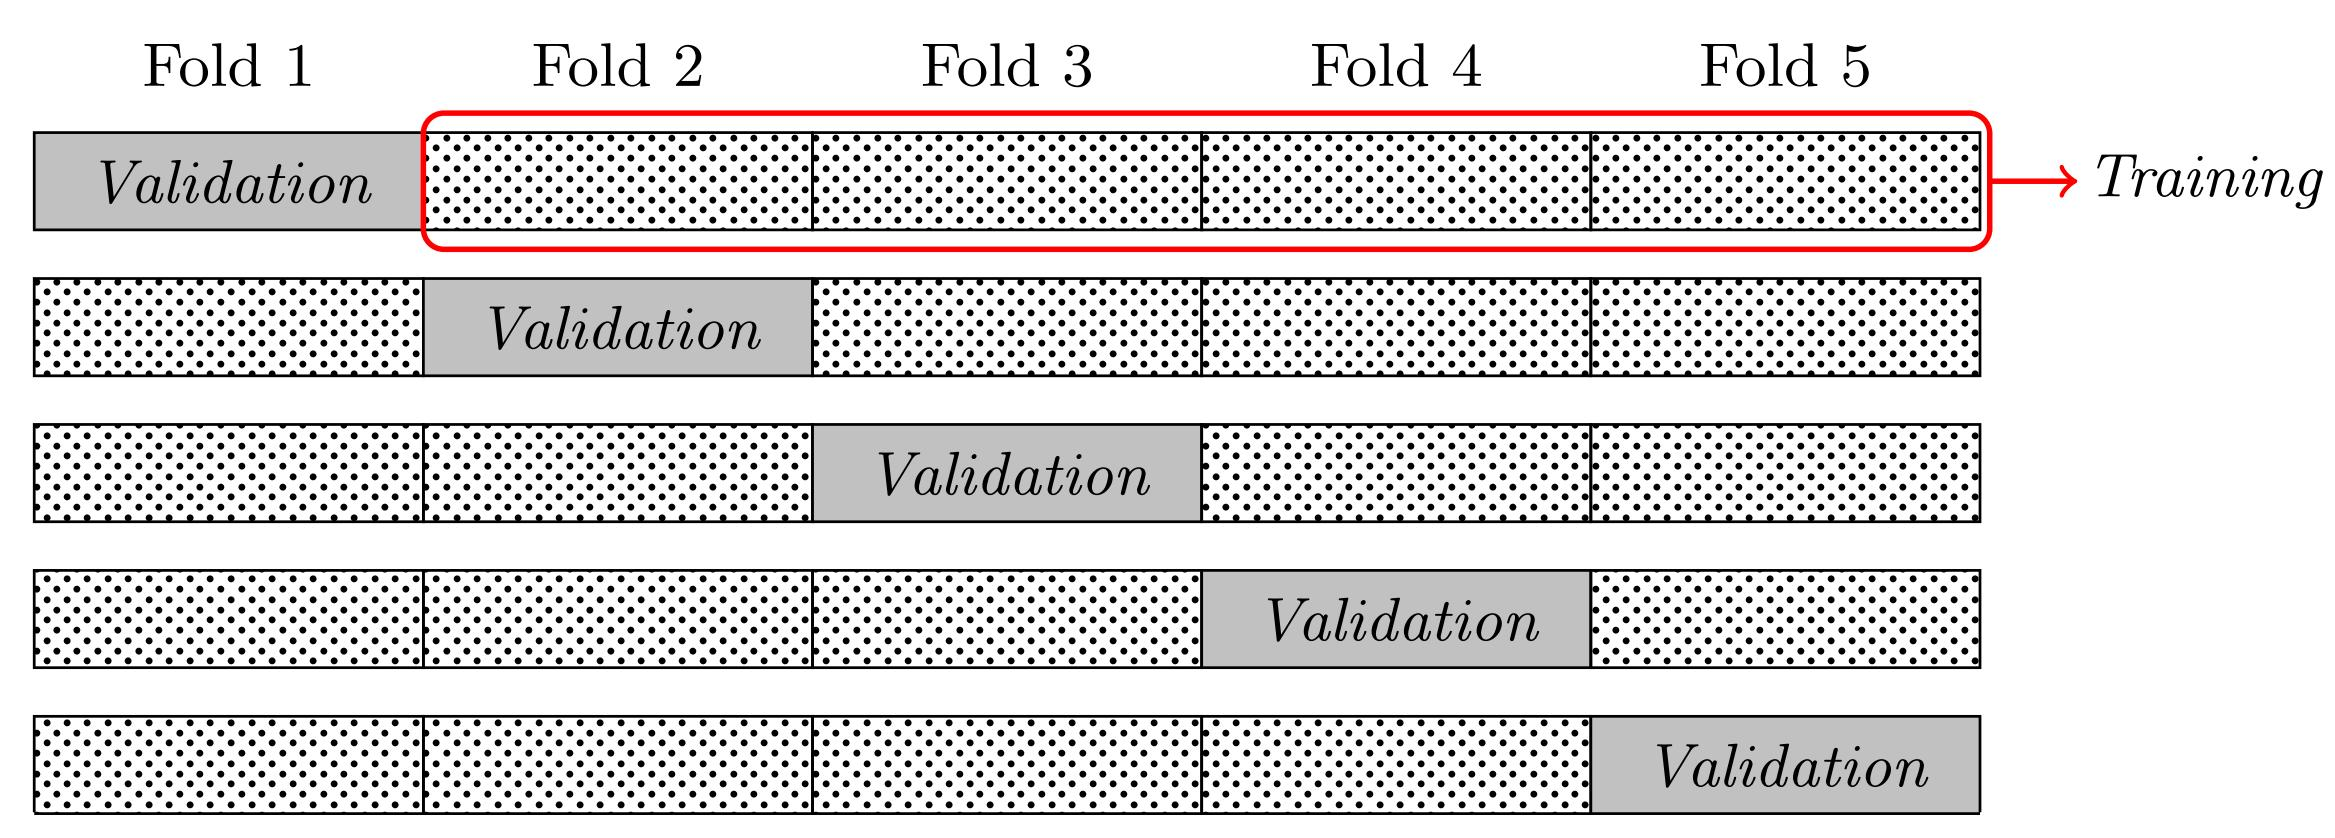
\includegraphics{figure/CV_f4_new.jpg}
			\end{figure}
		\end{center}
		
	\end{itemize}
\end{frame}





\begin{frame}{K-fold Cross Validation}{Step 2}
	\begin{itemize}
	\item[2] For each value of the tuning parameter $\lambda \in \{\lambda_{1},\ldots,\lambda_{m} \}$, we do the followings: 
				\vspace{0.2cm}
		\begin{itemize}
	\item Note that each $\lambda$ has the corresponding regression model so we have $m$ regression models in this case

		\end{itemize}
	
	
		
	\end{itemize}
\end{frame}



\begin{frame}{K-fold Cross Validation}{Step 2-1}
	\begin{itemize}
		\item[2-1] Compute the regression estimates $\mathrm{\hat{f}}^{-k}_{\lambda}$ using the \textbf{training data}
		\vspace{0.2cm}
		\begin{center}
			\begin{figure}[p]
				\centering
				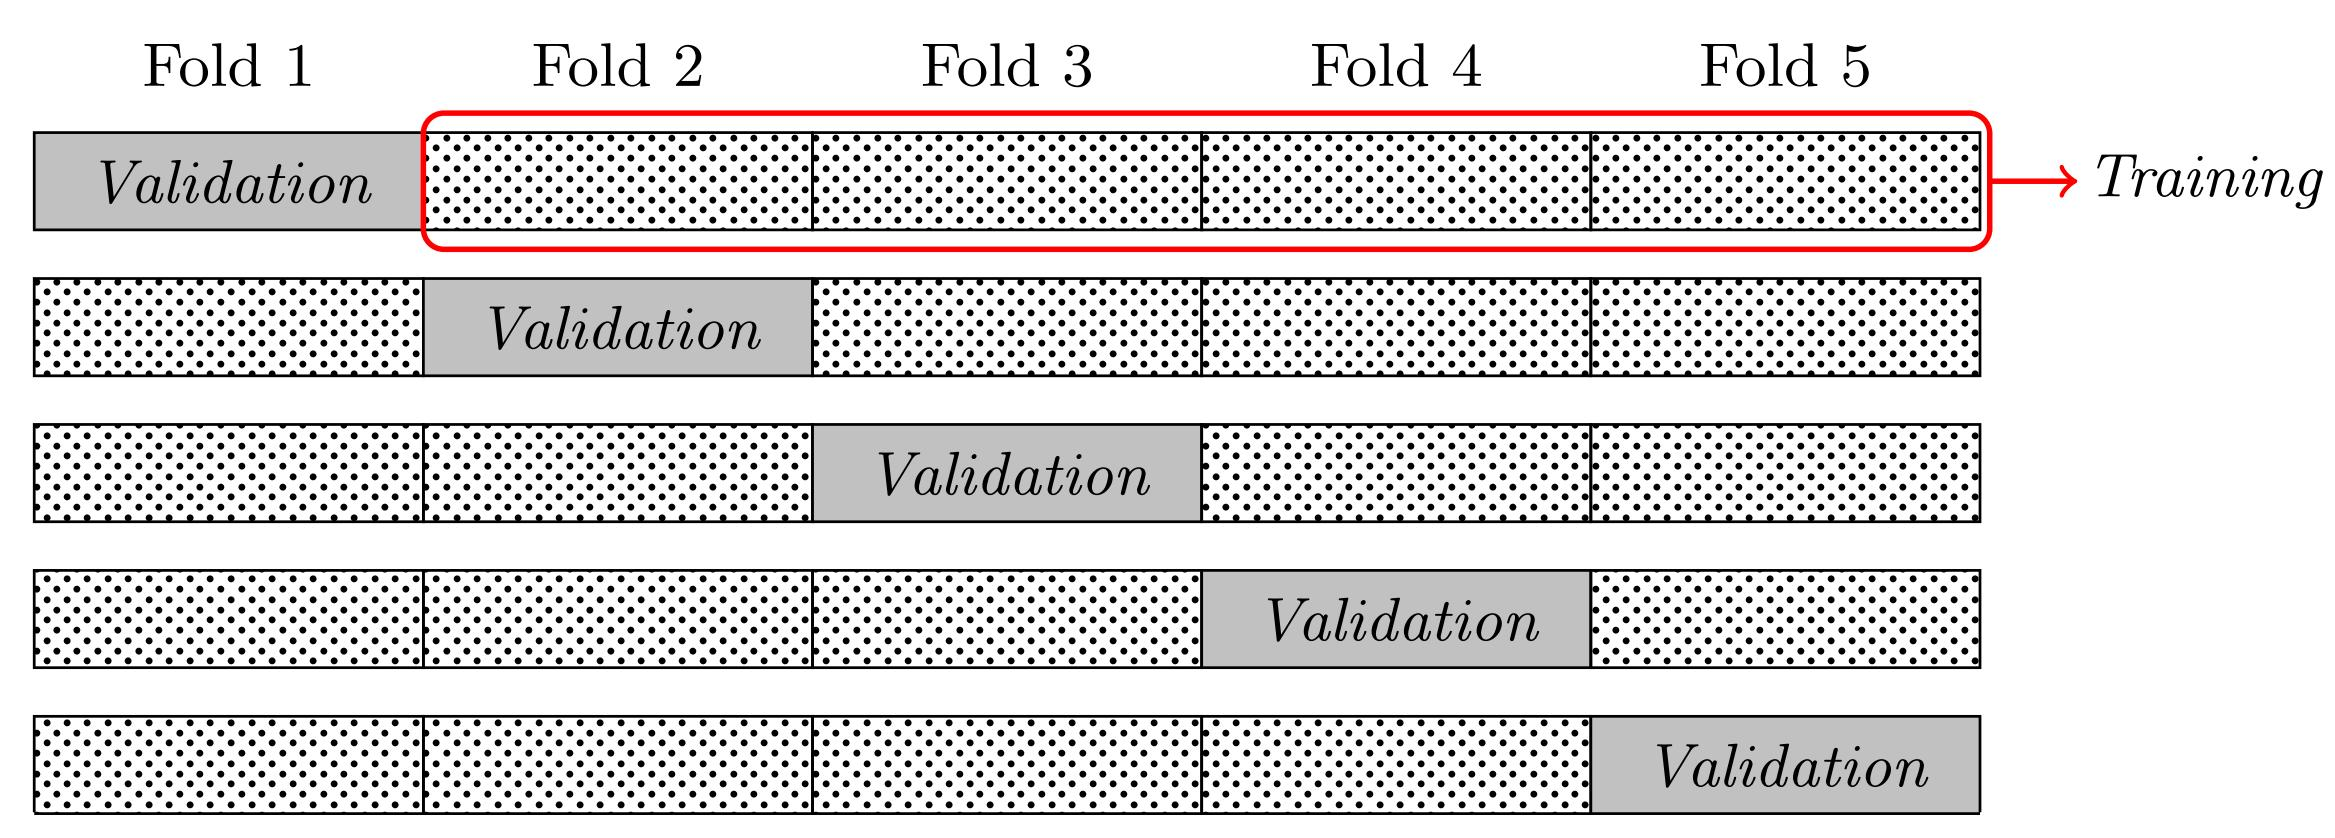
\includegraphics{figure/CV_f4_new.jpg}
			\end{figure}
		\end{center}
		
		
	\end{itemize}
\end{frame}



\begin{frame}{K-fold Cross Validation}{Step 2-2}
	\begin{itemize}
		\item[2-2] 
		Compute the prediction error $e_{k}(\lambda)$ on the each \textbf{validation data}:
	
			\begin{eqnarray*}
				e_{k}(\lambda) = \sum_{i \in F_{k}} (y^{+}_{i} - \mathrm{\hat{f}}^{-k}_{\lambda}(x^{j+}_{i}))^{2}
			\end{eqnarray*}
			
	\begin{center}
	\begin{figure}[p]
		\centering
		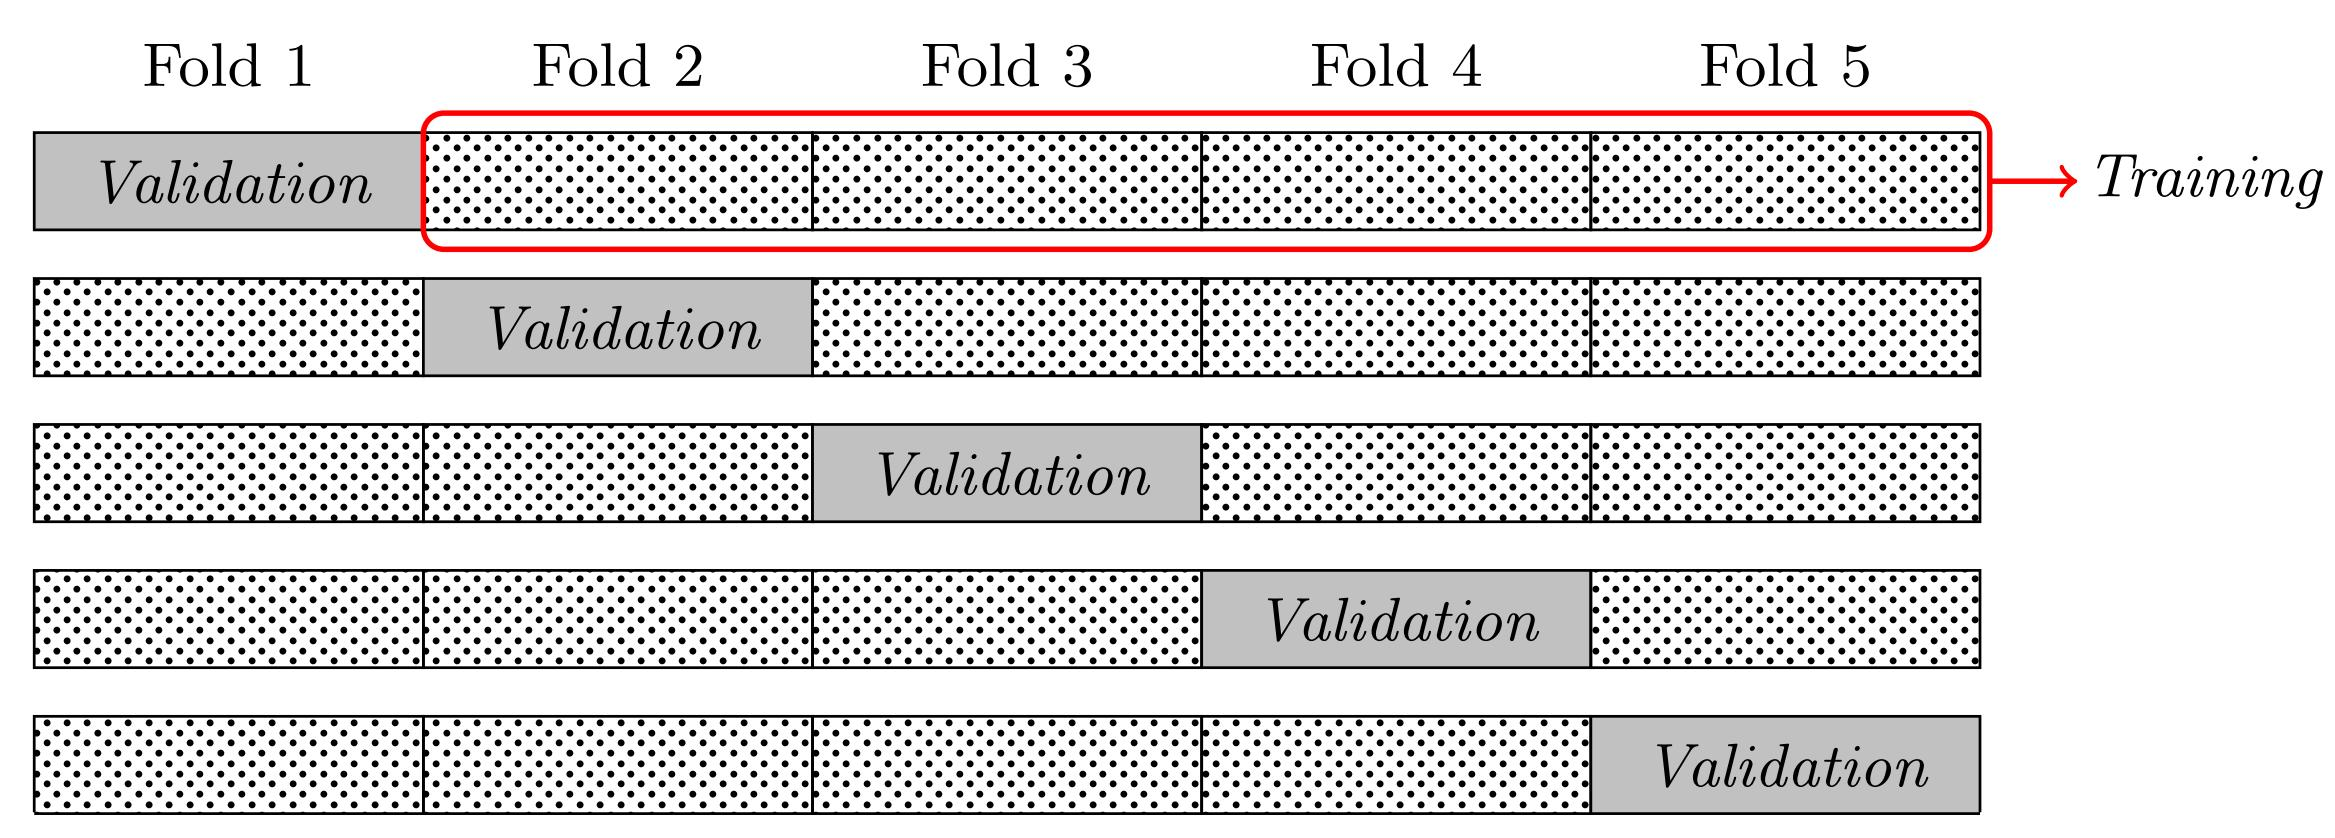
\includegraphics{figure/CV_f4_new.jpg}
	\end{figure}
\end{center}
		
		
	\end{itemize}
\end{frame}




\begin{frame}{K-fold Cross Validation}{Step 2-3}
	\begin{itemize}
		\item[2-3] Then, compute the \textbf{average prediction error}
	over all \textbf{validation data sets}
	\begin{eqnarray*}
		CV(\lambda) = \frac{1}{n} \sum^{K}_{k=1} e_{k}(\lambda) = \frac{1}{n} \sum^{K}_{k=1}  \sum_{i \in F_{k}} (y^{+}_{i} - \hat{f}^{-k}_{\lambda}(x^{j+}_{i}))^{2}
	\end{eqnarray*}
					
		\begin{center}
			\begin{figure}[p]
				\centering
				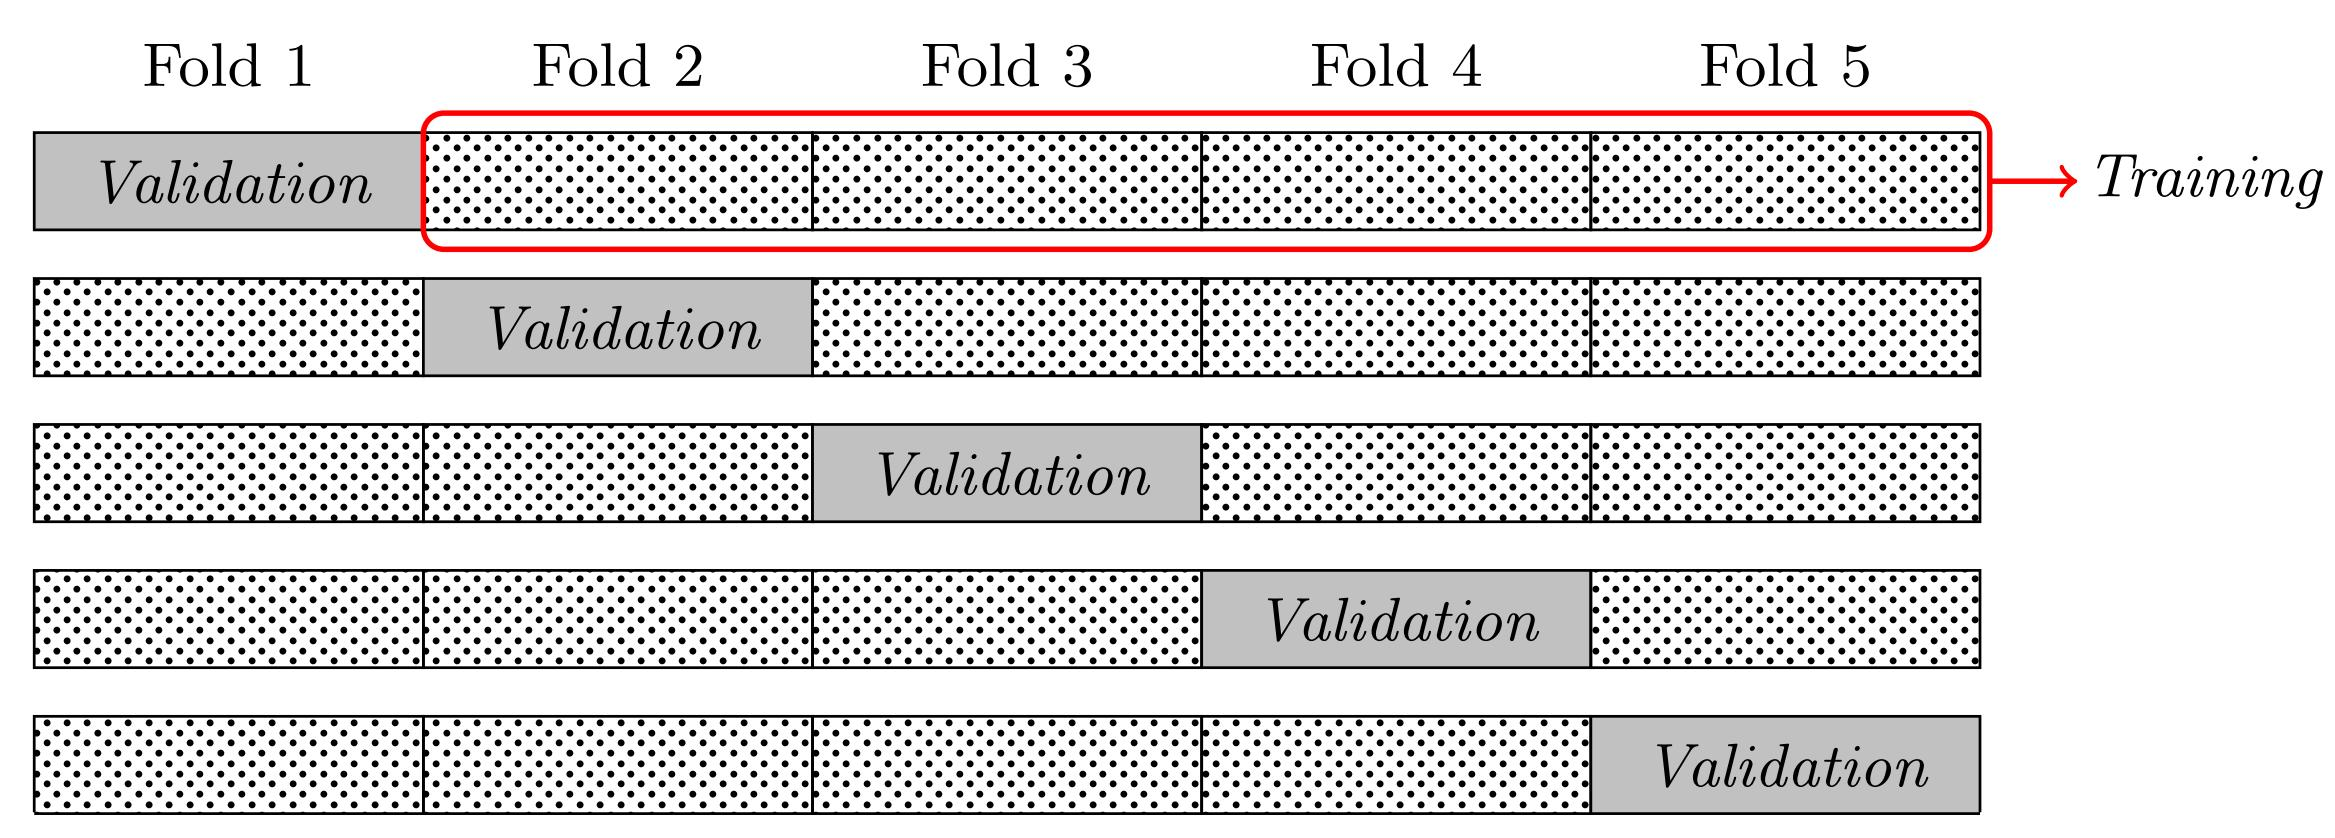
\includegraphics{figure/CV_f4_new.jpg}
			\end{figure}
		\end{center}
		
	\end{itemize}
\end{frame}





\begin{frame}{K-fold Cross Validation}{Step 2-3}
	\begin{itemize}
		\item[2-3] Having done this, we get a \textbf{average prediction error} $CV(\lambda)$ 
		\begin{itemize}	
						\vspace{0.2cm}
	\item It is also called \textbf{cross-validation error curve}
						\vspace{0.2cm}
	\item This curve is a function of $\lambda$	
			\end{itemize}
	\begin{center}
		\begin{figure}[p]
			\centering
			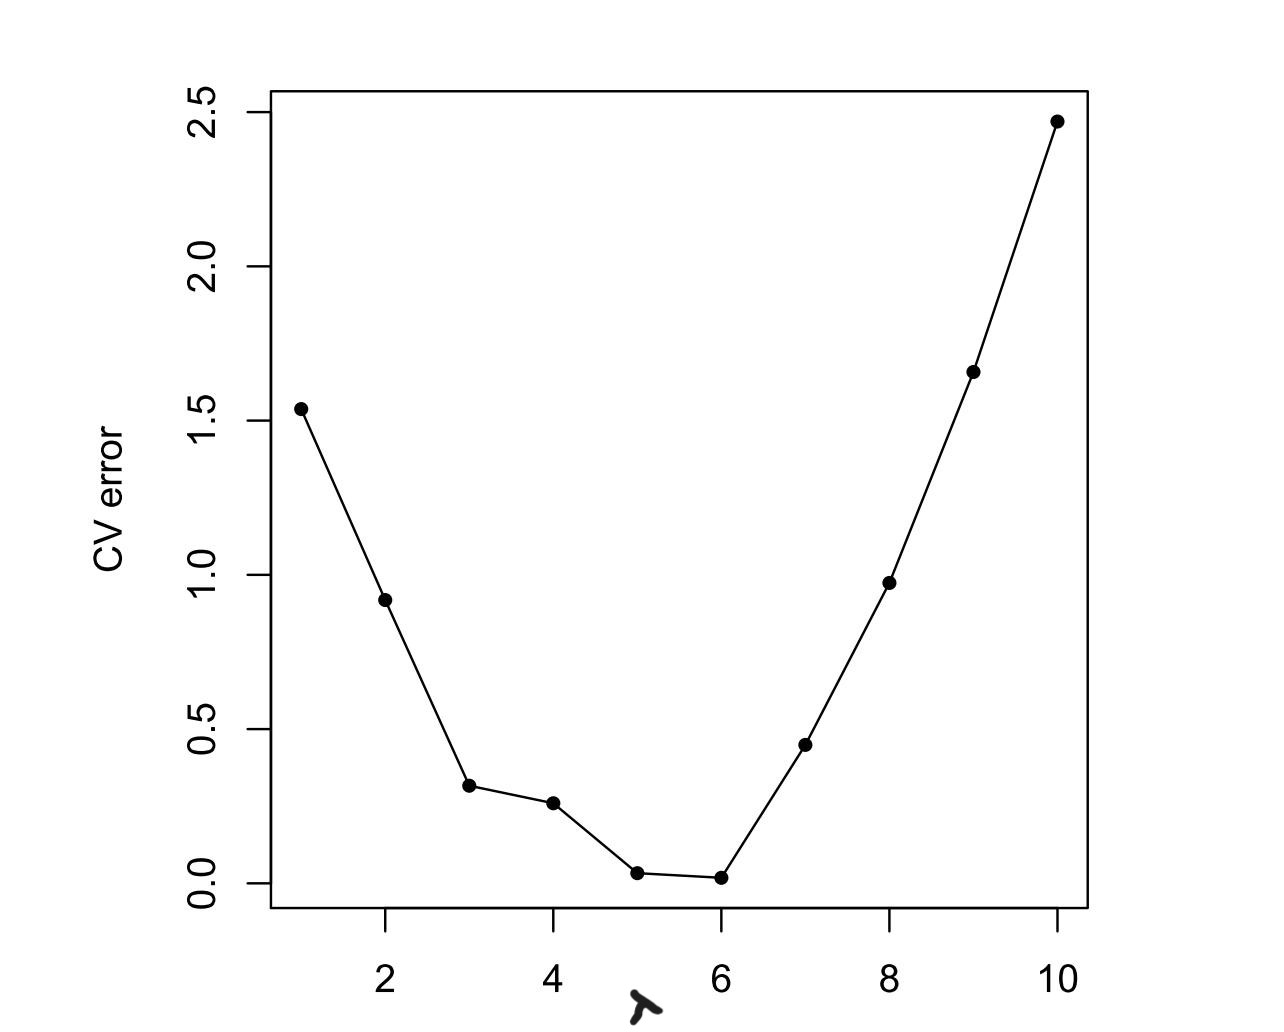
\includegraphics{figure/CV_f6.jpg}
		\end{figure}
	\end{center}
		
	\end{itemize}
\end{frame}





\begin{frame}{K-fold Cross Validation}{Step 3}
	\begin{itemize}
		\item[3] Choose the value of \textbf{tuning parameter} $\lambda$ that minimizes $CV(\lambda)$ curve: 
	\begin{eqnarray*}
		\hat{\lambda} = \arg \min_{\lambda \in \{ \lambda_{1},\ldots,\lambda_{m} \}} CV(\lambda)
	\end{eqnarray*}
	
	\item When $K = n$, we call this \textbf{leave-one-out cross-validation}, because we leave out one data point at a time
		
	\end{itemize}
\end{frame}







\begin{frame}{\textbf{Example:} 5-fold cross validation}

\begin{itemize}
			\begin{center}
		\begin{figure}[p]
			\centering
				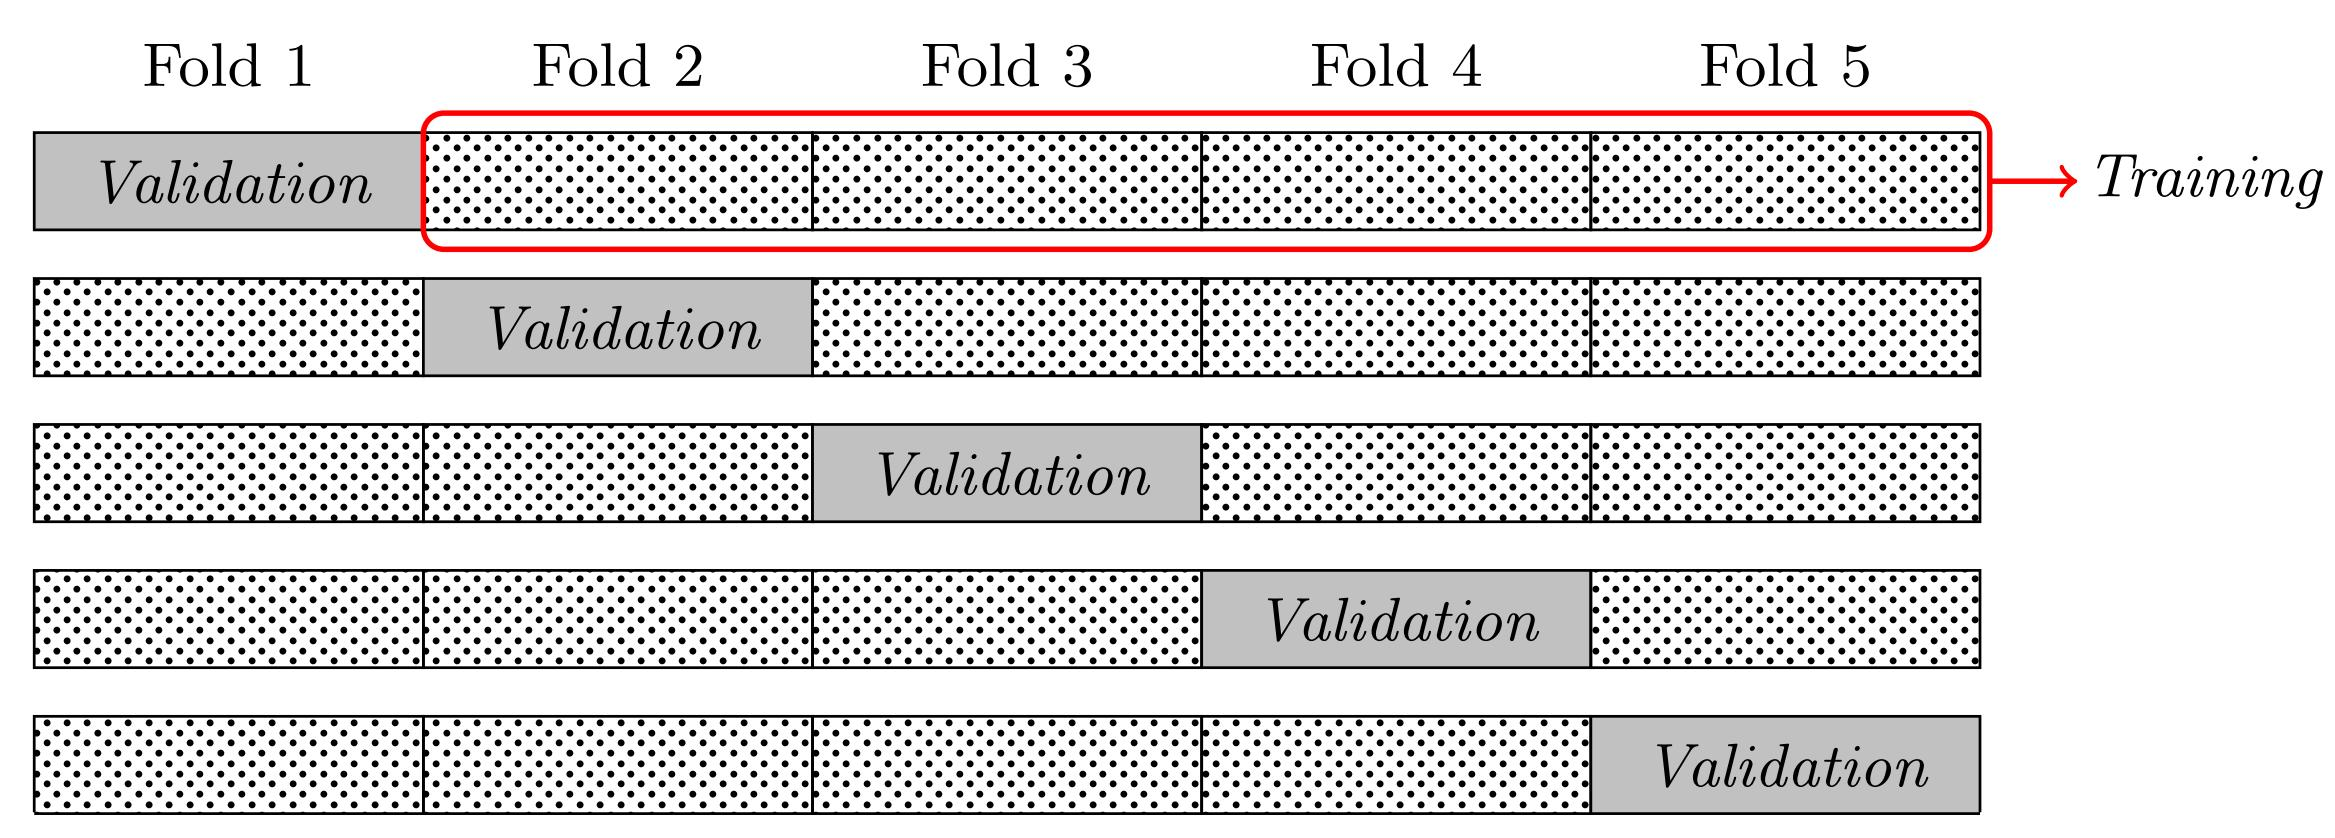
\includegraphics[width=0.8\textwidth]{figure/CV_f4_new.jpg}
			%
\includegraphics{CV_f4_new.jpg}
		\end{figure}
	\end{center}

	%\item \textbf{Example:} 5-fold cross validation
	\begin{itemize}
		\item[1] Pick 1st part of data as the \textbf{validation data} and use other parts of data as the \textbf{training data}
		\vspace{0.2cm}
		\item[2] For each value of the tuning parameter $\lambda \in \{\lambda_{1},\ldots,\lambda_{m} \}$, we do the followings: 
				\vspace{0.2cm}
			\begin{itemize}
		\item[2-1] Get estimated regression models based on \textbf{training data}
				\vspace{0.2cm}
		\item[2-2] Use these estimated regression models to predict each \textbf{validation data} and get \textbf{prediction errors}	
		\vspace{0.2cm}
		\item[2-3] Do the same thing for $k = 2,\ldots,5$ and get \textbf{average prediction errors}
		\vspace{0.2cm}
			\end{itemize}
		\item[3] Choose $\lambda$ that can minimize \textbf{average prediction errors} $CV(\lambda)$
	\end{itemize}
	
	
	%\vspace{0.2cm}
	%\item (When $K = n$, we call this \textbf{leave-one-out cross-validation}, because we leave out one data point at a time)
\end{itemize}
\end{frame}




\title[]  
{STATA Example}


\author 
{}

%\institute{Institute of Economics, Academia Sinica  \\ Econ, NTU}
%\institute{Institute of Economics, Academia Sinica  \\ IMES/IDAS, NCCU}
\institute{}

%\author 
%{楊子霆 \\ 中研院經濟所}

%\institute 
%{中正大學國際經濟專題研討}




\date
{}


\begin{frame}{}
	\titlepage
\end{frame}




\begin{frame}{STATA Example: Test the Convergence Hypothesis}{Overview}
		Sala-i-Martin, Xavier (1997), ``\textbf{I Just Ran Two Million Regressions}", American Economic Review
	
			\vspace{0.2cm}
	\begin{itemize}	
		\item The author tries to examine the hypothesis of growth convergence and the determinants of economic growth 
		\vspace{0.2cm}
		\begin{itemize}
			\item Whether poorer economies' per capita incomes will tend to grow at faster rates than richer economies
		\end{itemize}
		\vspace{0.2cm}
		\item He finds that a substantial number of variables can be found to be strongly related to growth
		\vspace{0.2cm}
		\item Citations: 2,931 times
		
	\end{itemize}
\end{frame}




\begin{frame}{STATA Example: Test the Convergence Hypothesis}{Overview}
	%Example 3: (Exogenous) Cross-Country Growth Regression.
	\begin{itemize}
		\item Examine the relation between GDP growth rate and initial per capita GDP: 
		\begin{eqnarray*}
			\underbrace{\mbox{GrowthRate}}_{Y_{i}} = \beta_{0} + \underbrace{\alpha}_{\mbox{ATE}} \underbrace{\log(\mbox{GDP})}_{D_{i}}	+ \sum^{p}_{j=1} \beta_{j} X^{j}_{i} + \epsilon_{i}	
		\end{eqnarray*}
		
        \item Control a lot of covariates $X^{j}_{i}$	
        
       \item In their data, they have $p = 60$ covariates, $n = 90$
        observations 
        				\vspace{0.2cm}
        	\begin{itemize}
        \item Need to do variable selection
        	\end{itemize}
		%where the model is exogenous,
		%\begin{eqnarray*}
		%	\mbox{E}[\epsilon|d_{i},x_{i}] =0.
		%\end{eqnarray*}
						\vspace{0.2cm}
		\item Test the convergence hypothesis $– \alpha < 0$ 
				\vspace{0.2cm}
		\begin{itemize}
		\item Poor countries catch up with richer countries, conditional on similar institutions etc. 
				\vspace{0.2cm}
		\item Prediction from the classical Solow growth model.   
		        	\end{itemize}
	
	\end{itemize}
\end{frame}




\begin{frame}[fragile]{STATA Example: Test the Convergence Hypothesis}{Data and Code}
	\begin{itemize}
	   \item See \textbf{ML.do}
		\vspace{0.2cm}
		\item Use growth.dta
		\vspace{0.2cm}
		
	\end{itemize}
\end{frame}




\begin{frame}[fragile]{STATA Example: Test the Convergence Hypothesis}{Control All Covariates}
\begin{lstlisting}
reg Outcome gdpsh465 bmp1l- tot1,r
\end{lstlisting}

\begin{itemize}	
	\item Control all 60 covariates	
	\vspace{0.2cm}
	\item This could result in imprecise estimates of coefficients due to overfitting
	%\vspace{0.2cm}
	%\item \textbf{fcstats}: display some statistics for evaluating the performance of model fitting
	
\end{itemize}


\end{frame}




\begin{frame}[fragile]{STATA Example: Test the Convergence Hypothesis}{Control All Covariates}
	\begin{itemize}
		\begin{figure}[p]
			\centering
			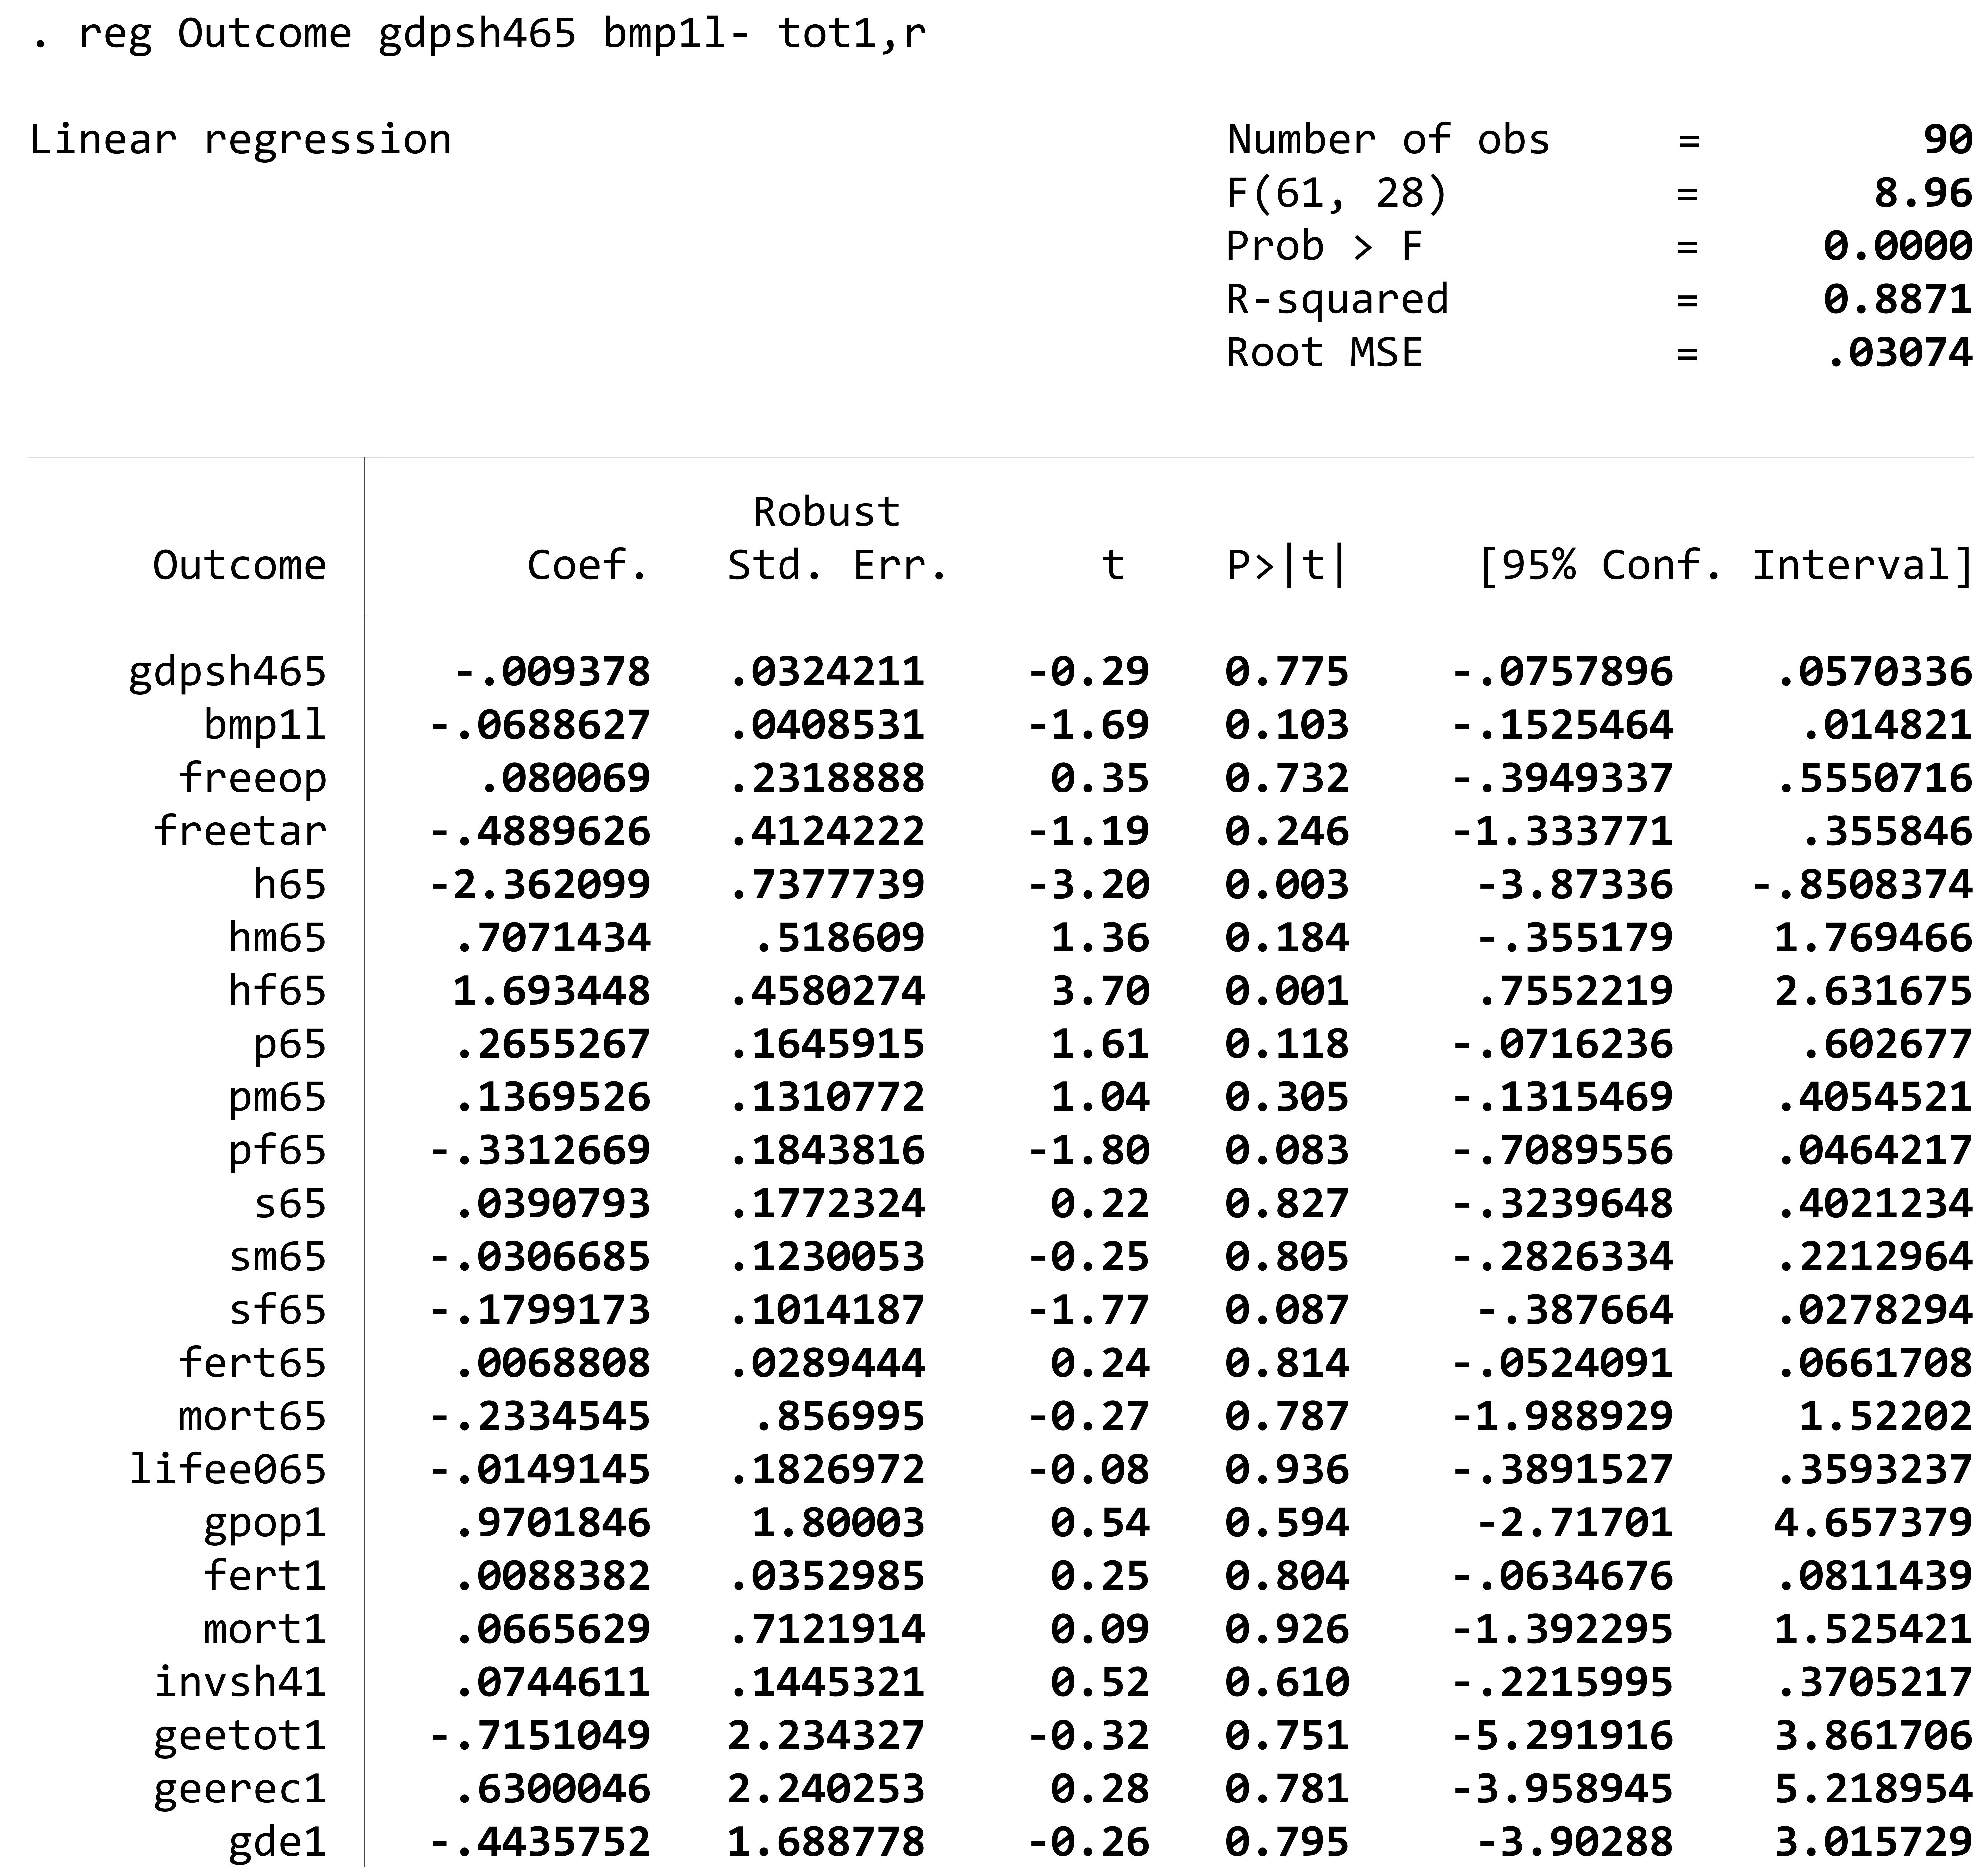
\includegraphics[width=.9\textwidth]{figure/growth_f1.jpg}
		\end{figure}
	\end{itemize}
\end{frame}



\begin{frame}[fragile]{STATA Example: Test the Convergence Hypothesis}{Control All Covariates}
\begin{itemize}	


\normalsize
\item The initial per capita GDP has little impact on economic growth rate	
\vspace{0.2cm}
\item Does NOT support prediction from the classical Solow growth model

\end{itemize}


\end{frame}





\begin{frame}{Review: Post-Double Selection Method}{Formal Illustration}

\begin{itemize}
\item Suppose the true model is:

\begin{eqnarray*}
	\underbrace{\mbox{GrowthRate}}_{Y_{i}} = \beta_{0} + \underbrace{\alpha}_{\mbox{ATE}} \underbrace{\log(\mbox{GDP})}_{D_{i}}	+ \sum^{p}_{j=1} \beta_{j} X^{j}_{i} + \epsilon_{i}	
\end{eqnarray*}




\end{itemize}

\end{frame}


\begin{frame}{Review: Post-Double Selection Method}{Formal Illustration}

\begin{itemize}



\item \textbf{Step 1:} Use ML methods (LASSO) to select covariates $X^{j}_{i}$ that can predict $Y_{i}$
\vspace{0.3cm}
\begin{itemize}
\item Denote the set of LASSO-selected covariates by A
\end{itemize}
%Suppose the treatment status $D$ is determined by:
\begin{eqnarray*}
\underbrace{\mbox{GrowthRate}}_{Y_{i}} = \delta_{0} + \sum^{p}_{j=1} \delta_{j} X^{j}_{i}  + \zeta_{i}
\end{eqnarray*}


\vspace{0.3cm}
\item \textbf{Step 2:} Use ML methods (LASSO) to select covariates $X^{j}_{i}$ that can predict $D_{i}$ 
\vspace{0.3cm}
\begin{itemize}
\item Denote the set of LASSO-selected covariates by B
\end{itemize}
\begin{eqnarray*}
\underbrace{\log(\mbox{GDP})}_{D_{i}} = \gamma_{0} +  \sum^{p}_{j=1} \gamma_{j} X^{j}_{i}  + \varepsilon_{i}
\end{eqnarray*}


\end{itemize}

\end{frame}



\begin{frame}{Review: Post-Double Selection Method}{Formal Illustration}
\begin{itemize}

\item \textbf{Step 3:} Estimate the following OLS regression:

\begin{eqnarray*}
\underbrace{\mbox{GrowthRate}}_{Y_{i}} = \pi_{0} + \underbrace{ \alpha}_{\mbox{ATE}}  D_{i} + \sum^{g}_{j=1} \pi_{j} U^{j}_{i}  + \upsilon_{i}
\end{eqnarray*}	

%\begin{eqnarray*}
%	D_{i} = \gamma_{0} +  \sum^{p}_{j=1} \gamma_{j} X^{j}_{i}  + \varepsilon_{i} \\
%	Y_{i} = \delta_{0} + \sum^{p}_{j=1} \beta_{j} X^{j}_{i}  + \zeta_{i}
%\end{eqnarray*}	





%\item PDS method starts by fitting LASSO regression models to both (2) and (3)	
%	\vspace{0.3cm}
\begin{itemize}
\item Let $U^{j}_{i}$ denote the \textbf{union of covariates in A and B}
\end{itemize}
\vspace{0.3cm}
\item The PDS estimator of treatment effect $\alpha$ is the coefficient on $D$ in the above OLS regression
\vspace{0.2cm}
	\item The additional selection step 2 can help eliminate the \textbf{omitted variable bias}



\end{itemize}



\end{frame}





\begin{frame}{Review: Three Ways to Choose $\lambda$}{Overview}
	\begin{itemize}
		\item[1] \textbf{Cross-validation approach:} It is a data-driven approach. Choose \textbf{tuning parameter} $\lambda$ that minimize \textbf{prediction
			error}
		\vspace{0.2cm}
			\begin{itemize}
		\item STATA command: \textbf{cvlasso}
			\end{itemize}
				\vspace{0.2cm}
		\item[2] \textbf{Rigorous approach:} It is a theory-driven approach. Belloni et al. (2012, Econometrica) develop theory and feasible algorithms for the optimal $\lambda$.
			\vspace{0.2cm}
		\begin{itemize}
			\item STATA command: \textbf{rlasso}
		\end{itemize}

		\vspace{0.2cm}
		\item[3] \textbf{Information criteria approach:} Select the value of $\lambda$ that minimizes information criterion (AIC, AICc, BIC or EBIC
).
			\vspace{0.2cm}
		\begin{itemize}
			\item STATA command: \textbf{lasso2}
		\end{itemize}
		%Cross-validation is a simple, intuitive way to evaluate model fit (choose $\lambda$) based on \textbf{prediction
		%error}
					\vspace{0.2cm}
		\item To use the above commands, you need to install \textbf{lassopack} package
			\vspace{0.2cm}
		\begin{itemize}
			\item STATA command: \textbf{ssc install lassopack}
		\end{itemize}
		
		
	\end{itemize}
\end{frame}








\begin{frame}[fragile]{STATA Example: Test the Convergence Hypothesis}{Use Post-Double Selection Method}
\begin{lstlisting}
pdslasso Outcome gdpsh465 (bmp1l- tot1),rob
  \end{lstlisting}
	
	\begin{itemize}	
		\item \textbf{pdslasso}: Implement double selection method with LASSO to select covariates
		\vspace{0.2cm}
			\begin{itemize}	
		\item Select covariates from $bmp1l- tot1$ to predict outcome $Y_{i}$ and treatment variable $D_{i}$
			\end{itemize}
				%\vspace{0.2cm}
		%\item Instead of 60 variables, this method only select 10 variables that are correlated with both outcome $Y_{i}$ and treatment variable $D_{i}$
		%\vspace{0.2cm}
		%\item \textbf{fcstats}: display some statistics for evaluating the performance of model fitting
		
	\end{itemize}
	
	
\end{frame}





\begin{frame}[fragile]{STATA Example: Test the Convergence Hypothesis}{Use Post-Double Selection Method}
	\begin{itemize}
		\begin{figure}[p]
			\centering
			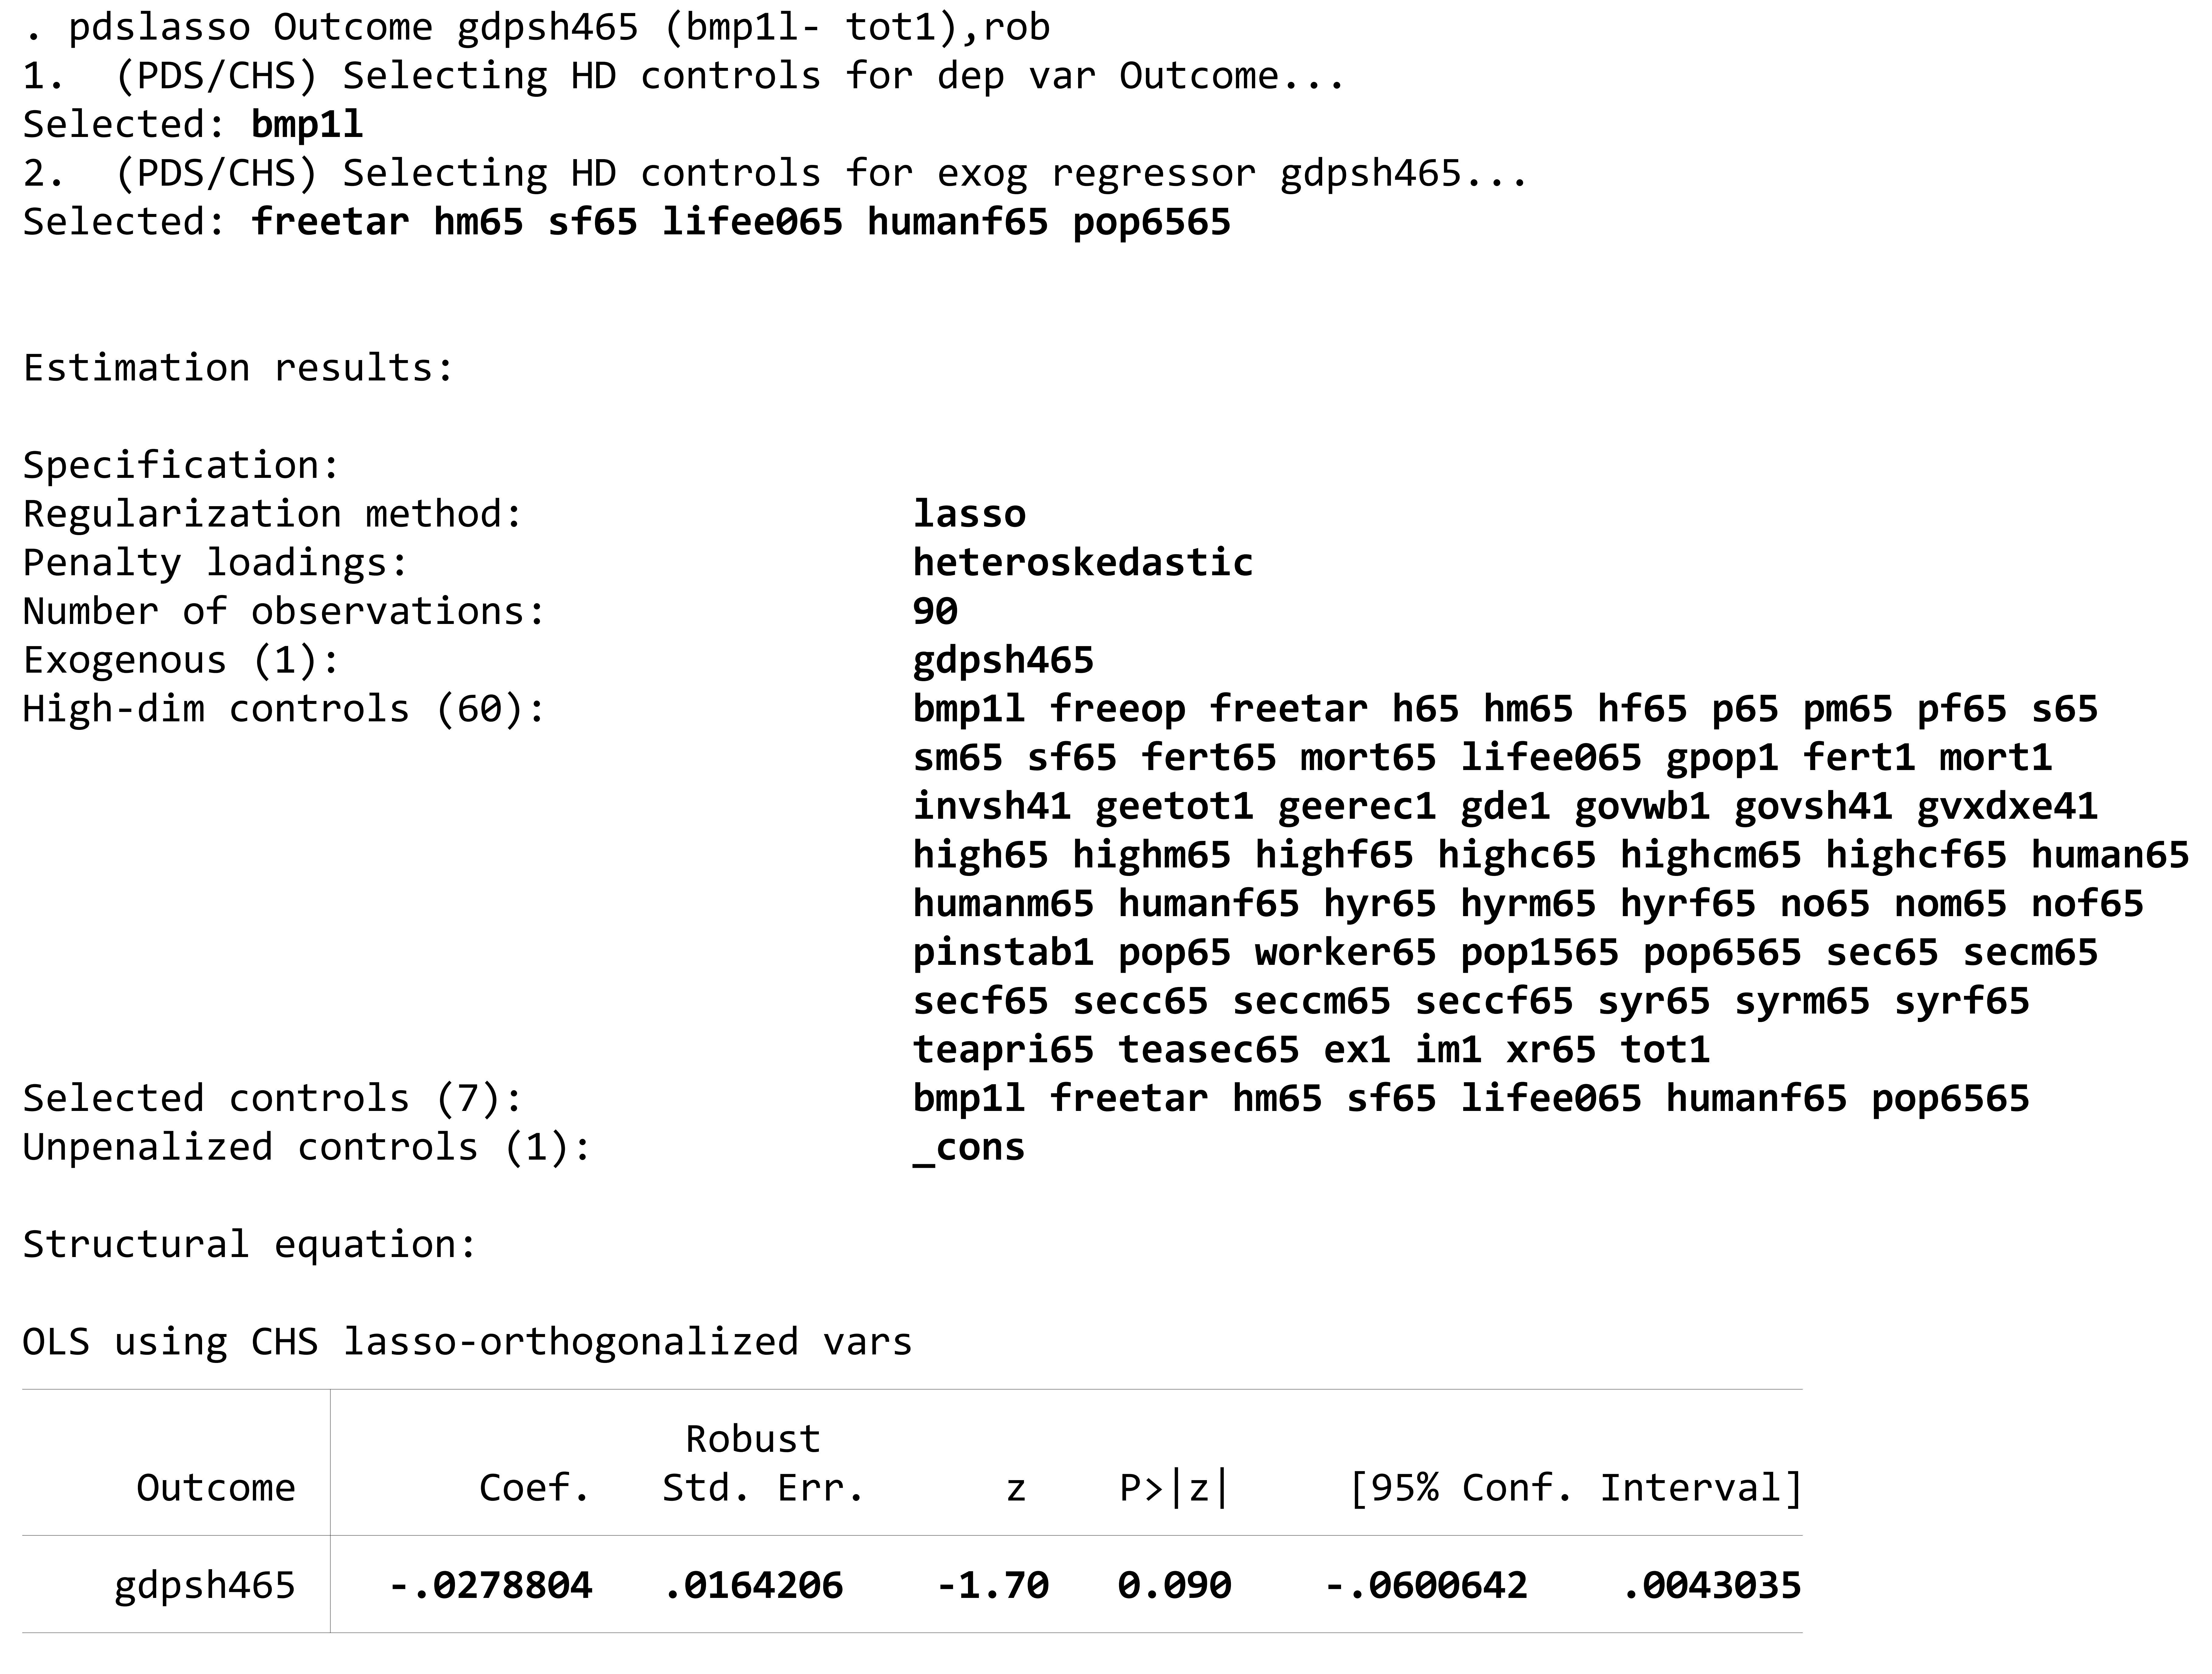
\includegraphics[width=.8\textwidth]{figure/growth_f2.jpg}
		\end{figure}
	\end{itemize}
\end{frame}







\begin{frame}[fragile]{STATA Example: Test the Convergence Hypothesis}{Use Post-Double Selection Method}
	\begin{itemize}
		\begin{figure}[p]
			\centering
			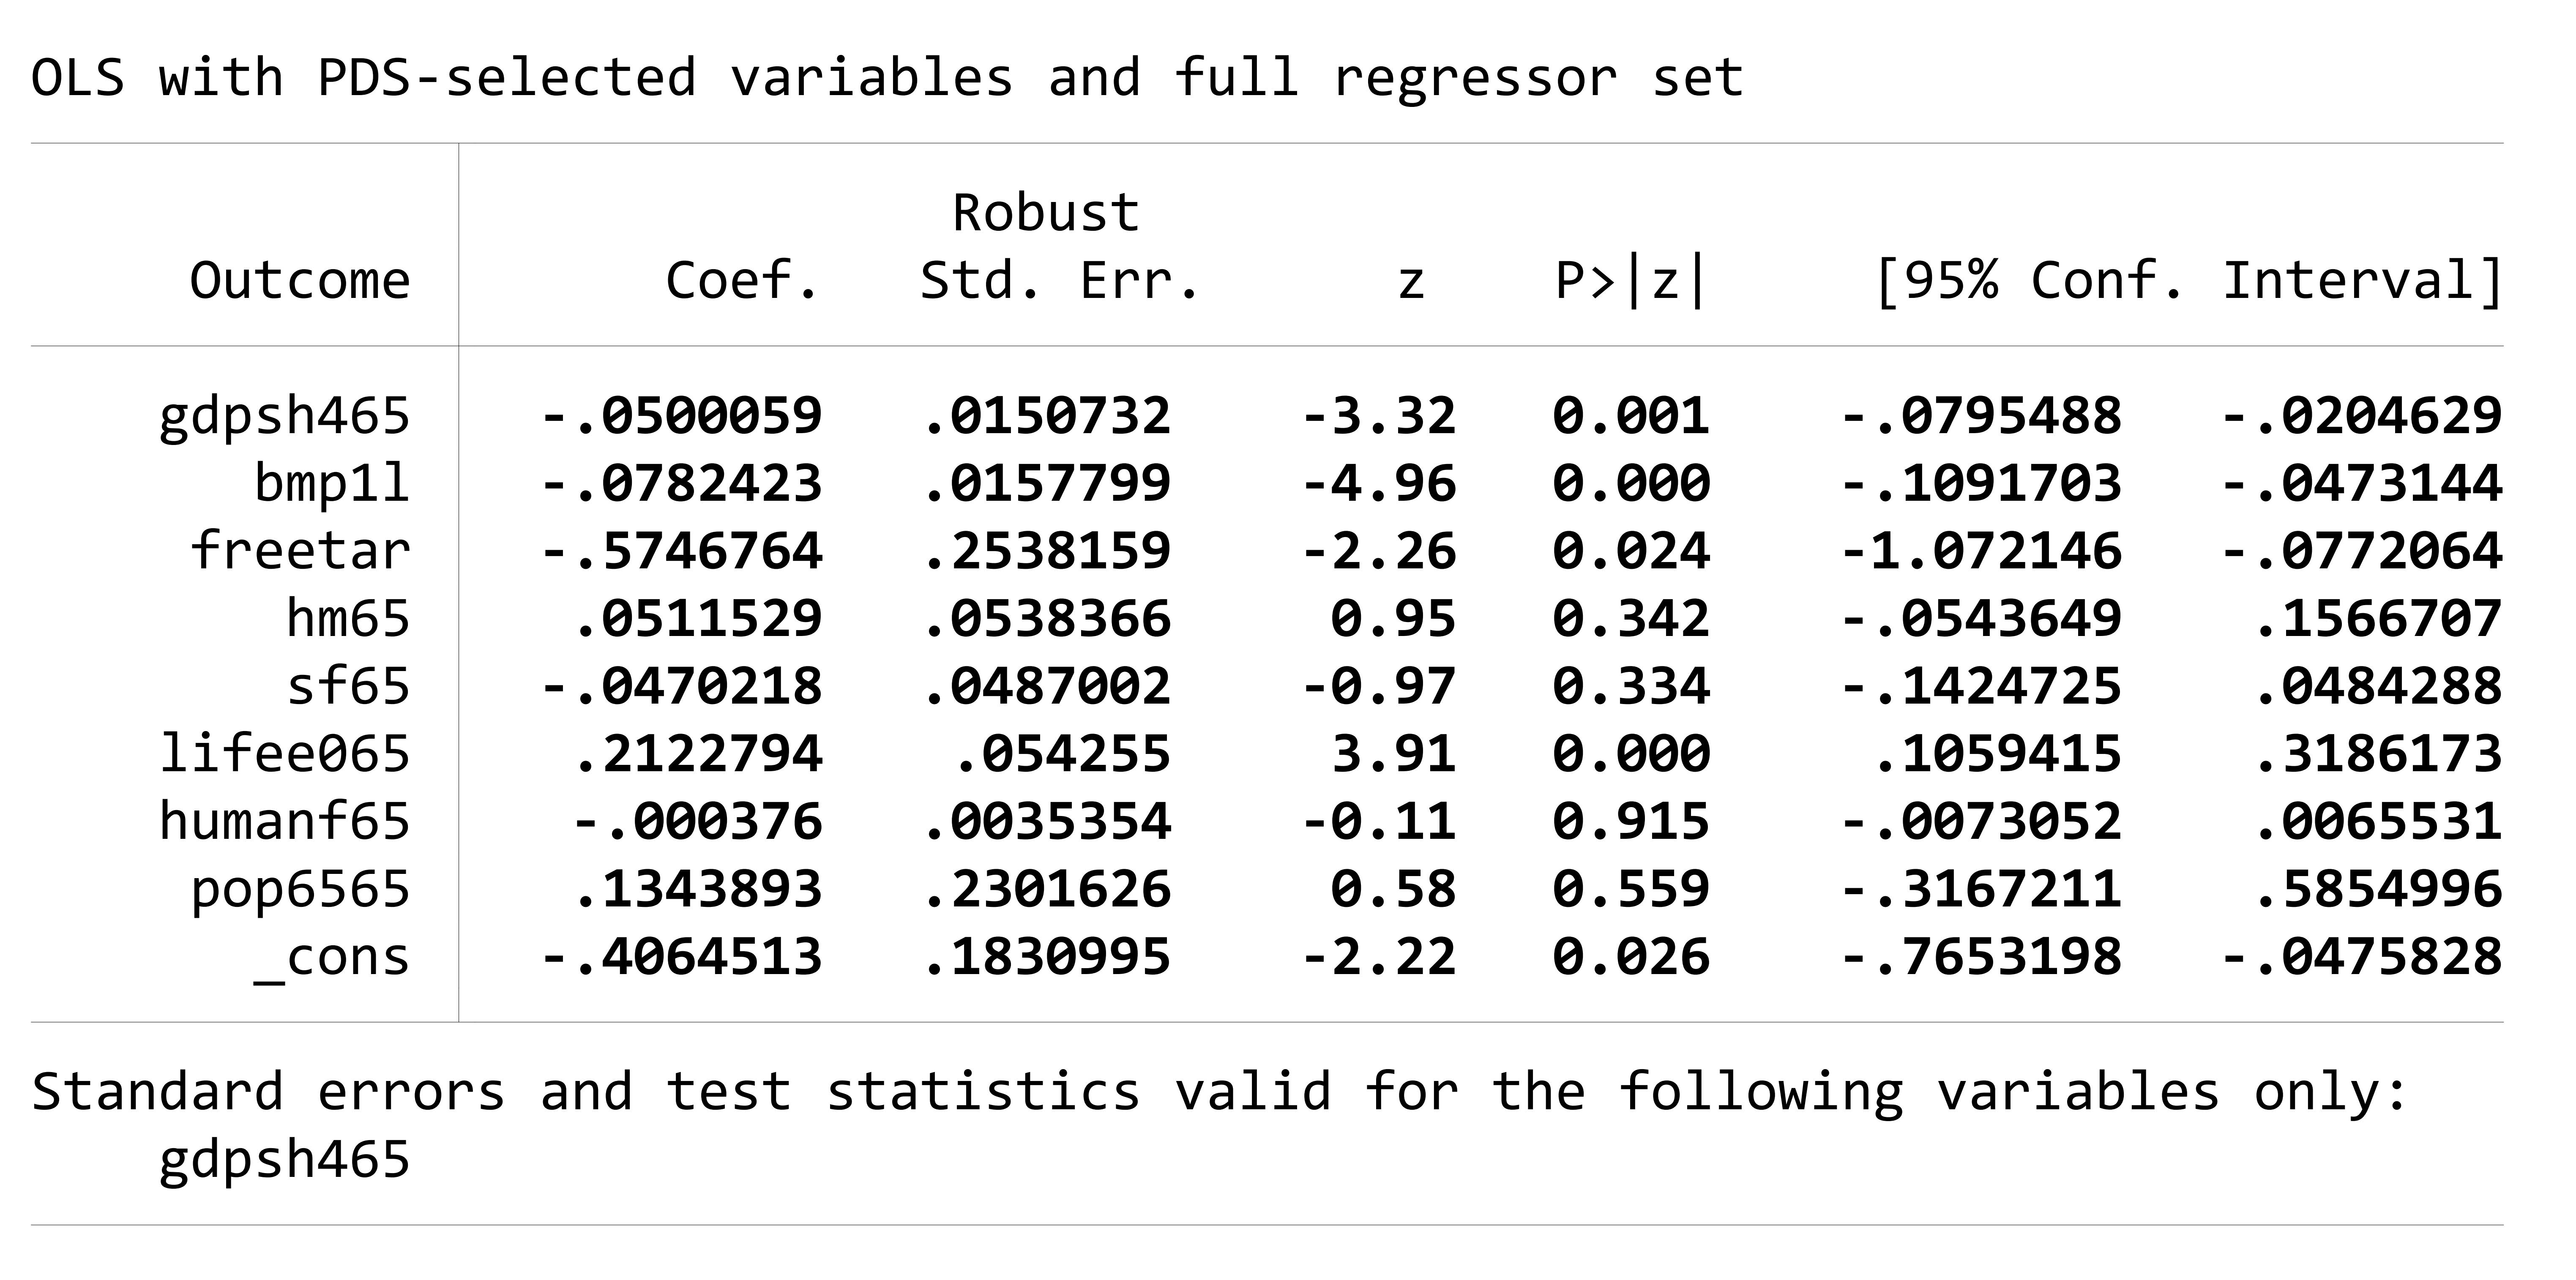
\includegraphics[width=.9\textwidth]{figure/growth_f3.jpg}
		\end{figure}
	\end{itemize}
\end{frame}



\begin{frame}[fragile]{STATA Example: Test the Convergence Hypothesis}{Use Post-Double Selection Method}
		
	
	\begin{itemize}	
		\vspace{0.2cm}
		\normalsize
		\item Instead of 60 variables, this method only select 7 variables that are correlated with outcome $Y_{i}$ or treatment variable $D_{i}$
		%\vspace{0.2cm}
		%\item \textbf{fcstats}: display some statistics for evaluating the performance of model fitting
		\vspace{0.2cm}
			\begin{itemize}	
				\item Higher initial per capita GDP could lead to lower GDP growth rate in the later years
		\vspace{0.2cm}
		\item Poor countries do catch up with richer countries
				\vspace{0.2cm}
					\end{itemize}
	    \item Support prediction from the classical Solow growth model

	\end{itemize}
	
	
\end{frame}



\begin{frame}[fragile]{STATA Example: Test the Convergence Hypothesis}{Use Post-Double Selection Method}
\begin{lstlisting}
** step 1: 
rlasso Outcome bmp1l- tot1,rob

** step 2: 
rlasso gdpsh465 bmp1l- tot1,rob

** step 3:
reg Outcome gdpsh465 bmp1l freetar hm65 sf65 lifee065 humanf65 pop6565,r

\end{lstlisting}
	
	\begin{itemize}	
	\item You can implement PDS method by yourself
		\vspace{0.2cm}
	\item PDS uses rigorous approach to select optimal $\lambda$.
	\vspace{0.2cm}
	\begin{itemize}
		\item STATA command: \textbf{rlasso}
	\end{itemize}


	\end{itemize}
	
	
\end{frame}




\begin{frame}[fragile]{STATA Example: Test the Convergence Hypothesis}{Use Post-Double Selection Method}
\begin{lstlisting}
pdslasso Outcome gdpsh465 (bmp1l- tot1), rob pnotpen(ex1 im1)
\end{lstlisting}
	
	\begin{itemize}    
		\item \textbf{pnotpen(ex1 im1)}: Specifies variables that are automatically included in the model without going through the selection process
		\vspace{0.2cm}
			\begin{itemize}
		\item Variables in \textbf{pnotpen()} are not penalized and will always be included in the final model, regardless of their statistical significance
			\end{itemize}
	\end{itemize}
	
\end{frame}








\begin{frame}[fragile]{STATA Example: Visualize Data}{Scatter Plot}
\begin{lstlisting}
graph twoway ///
(scatter Outcome gdpsh465) ///
(lfit Outcome gdpsh465), ///
title("GDP Growth Rate (2000) vs. log(GDP) (1965)") ///
xtitle("log(GDP) in 1965") ///
ytitle("GDP Growth Rate in 2000") ///
graphregion(color(white)) xlabel(5(1)10) ylabel(-0.1(0.1)0.2)

graph export "$pic\gdp_scatter.png", replace width(3000)
\end{lstlisting}
	\begin{itemize}	
 \item \textbf{graph twoway scatter}
\begin{itemize}
	\item Generates a scatter plot with `Outcome` as the y-axis and `gdpsh465` as the x-axis.
\end{itemize}
	\vspace{0.2cm}
\item \textbf{graphregion(color(white))} 
\begin{itemize}
	\item Sets the background color of the graph to white for a clean look.
\end{itemize}
	\vspace{0.2cm}
\item \textbf{graph export} 
\begin{itemize}
	\item Exports the graph as a PNG file named
\end{itemize}
		
		
	\end{itemize}
	
\end{frame}

\begin{frame}[fragile]{STATA Example: Visualize Data}{Scatter Plot}
	\begin{itemize}
		\begin{figure}[p]
			\centering
			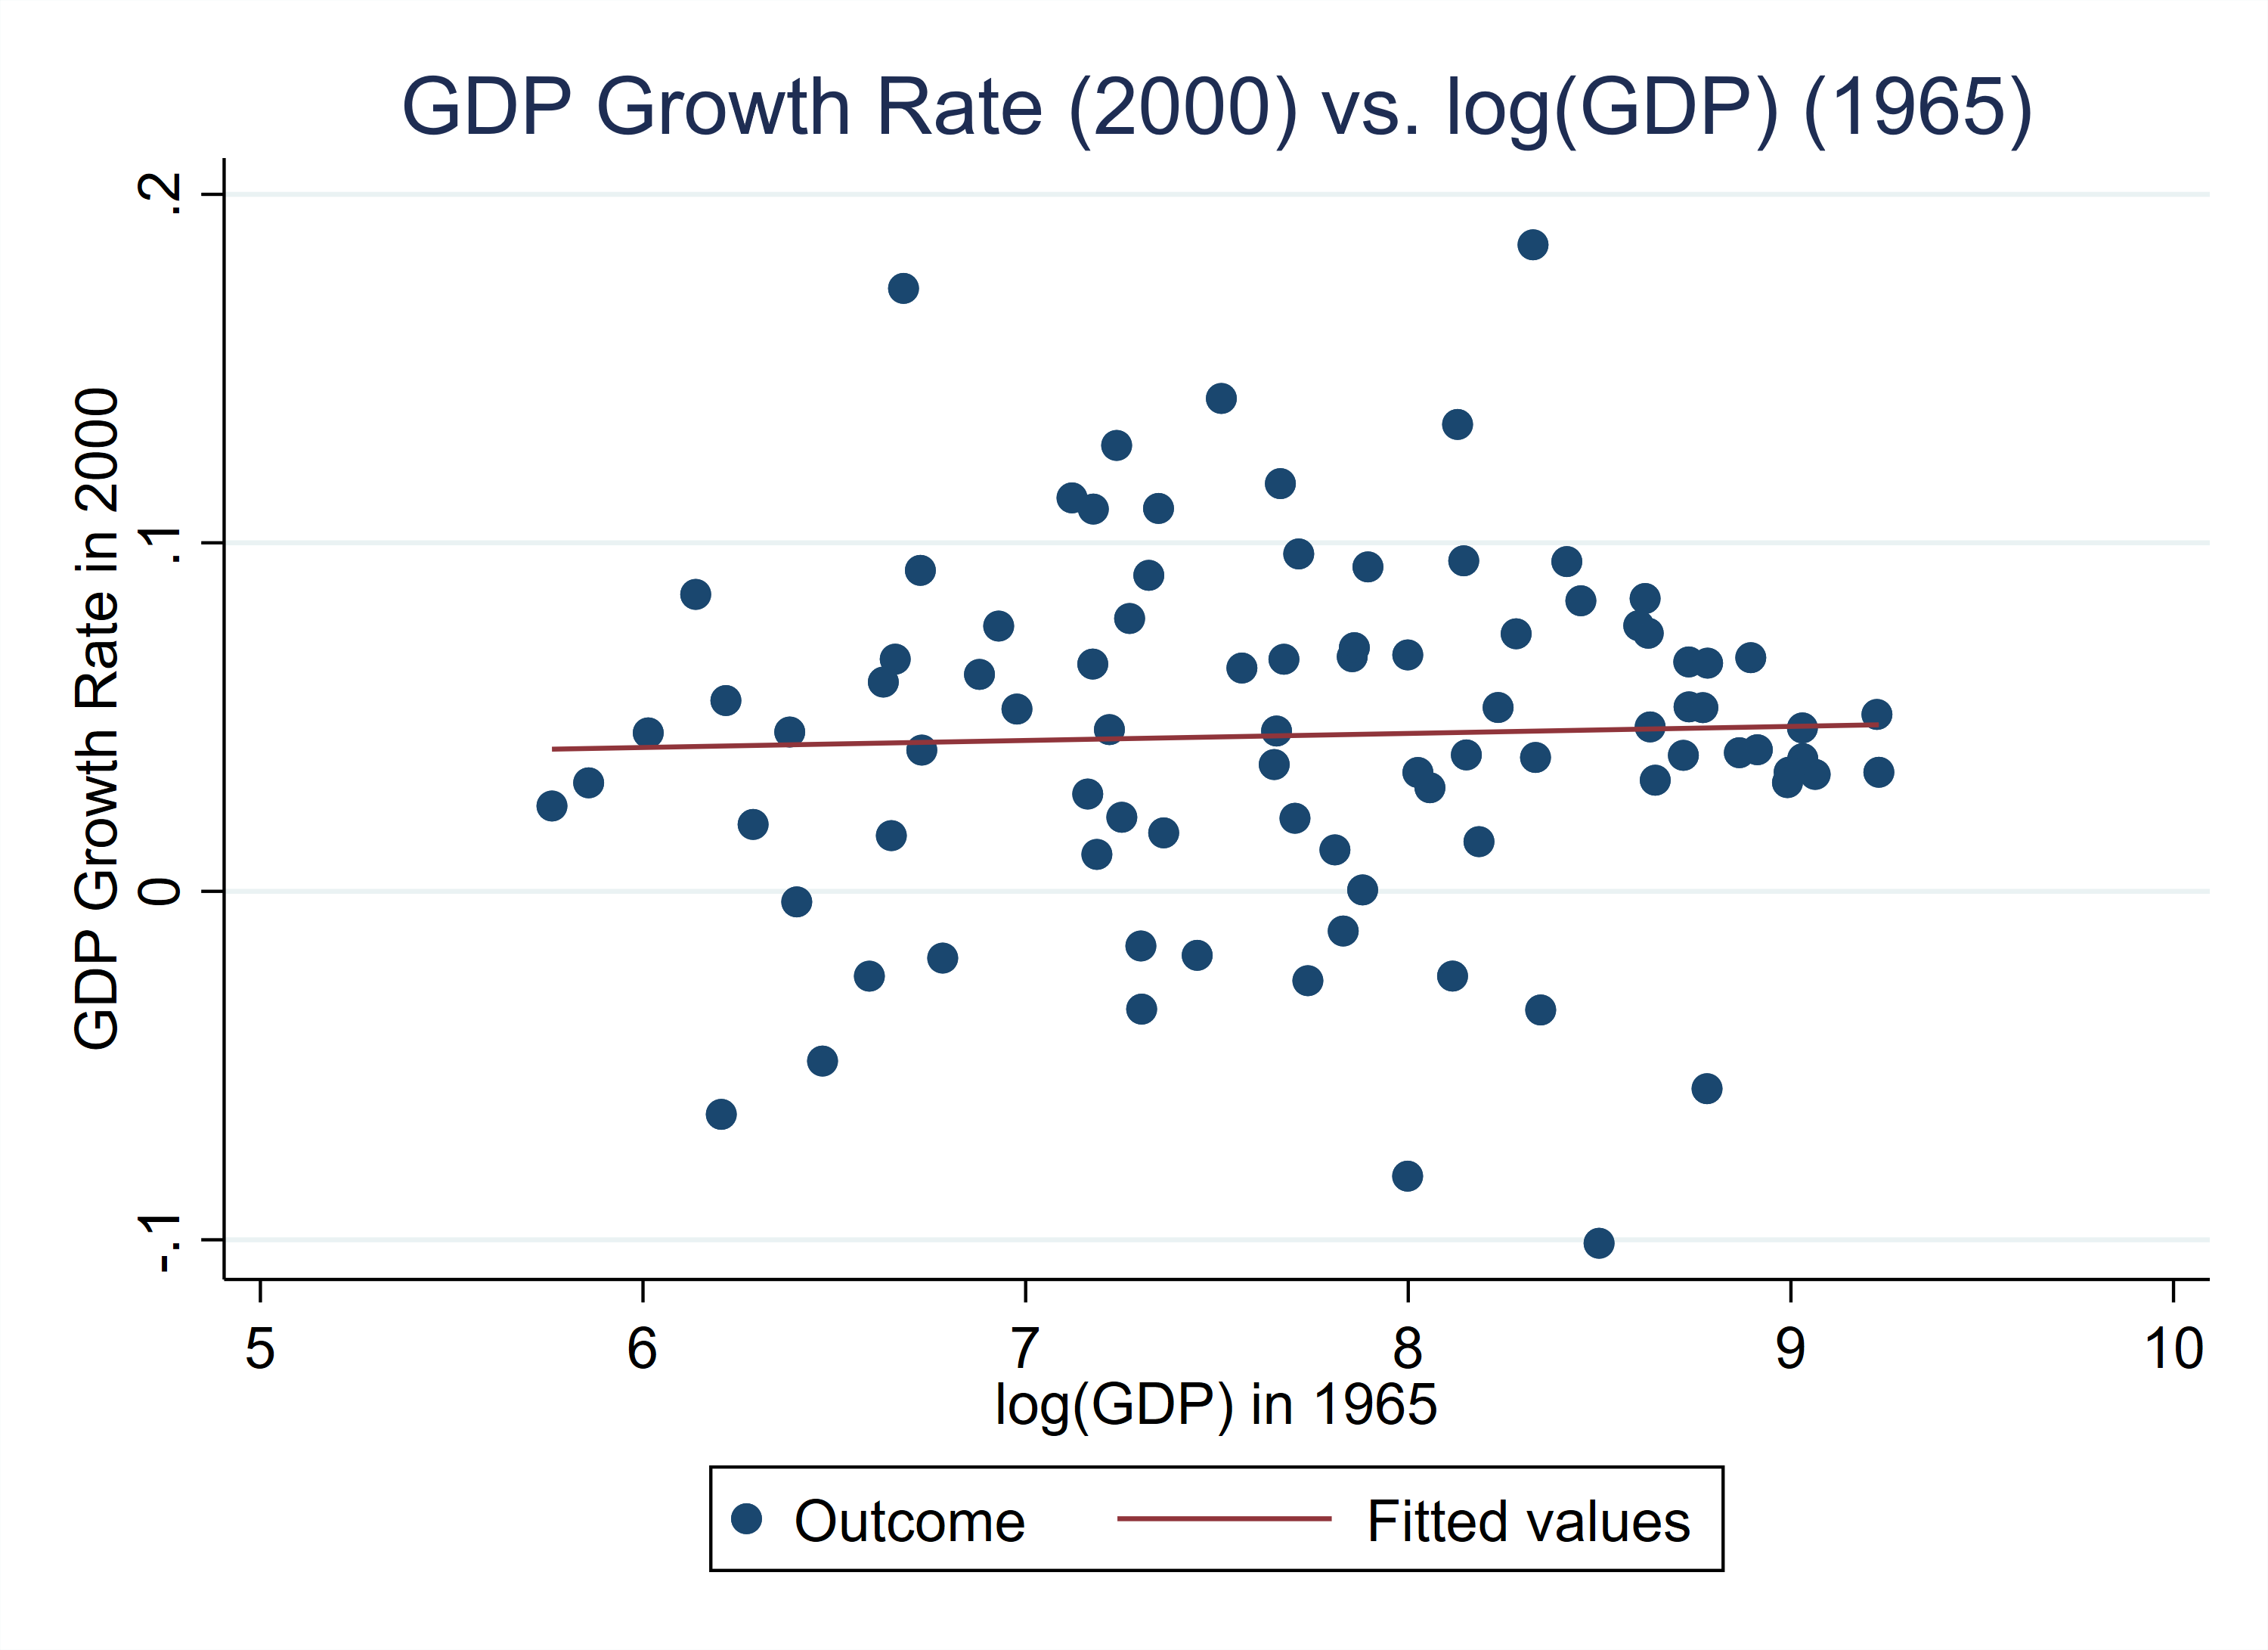
\includegraphics[width=.8\textwidth]{figure/gdp_scatter.png}
		\end{figure}
	\end{itemize}
\end{frame}




\begin{frame}[fragile]{STATA Example: Visualize Data}{Scatter Plot: residuals}
\begin{lstlisting}
* Regress Outcome on control variables and get residuals
regress Outcome bmp1l freetar hm65 sf65 lifee065 humanf65 pop6565
predict res_Outcome, residuals

* Regress gdpsh465 on control variables and get residuals
regress gdpsh465 bmp1l freetar hm65 sf65 lifee065 humanf65 pop6565
predict res_gdpsh465, residuals
\end{lstlisting}

	
\end{frame}



\begin{frame}[fragile]{STATA Example: Visualize Data}{Scatter Plot: residuals}
\begin{lstlisting}
* Scatter plot of the residuals
graph twoway ///
(scatter res_Outcome res_gdpsh465) ///
(lfit res_Outcome res_gdpsh465), ///
title("Partialed Scatter Plot of Outcome vs. gdpsh465") ///
xtitle("Residual log(GDP) in 1965") ///
ytitle("Residual GDP Growth Rate in 2000") ///
graphregion(color(white)) xlabel(-1(0.5)1) ylabel(-0.1(0.1)0.2)

graph export "$pic\gdp_scatter_r.png", replace width(3000)
\end{lstlisting}
	
	
\end{frame}


\begin{frame}[fragile]{STATA Example: Visualize Data}{Scatter Plot: residuals}
	\begin{itemize}
		\begin{figure}[p]
			\centering
			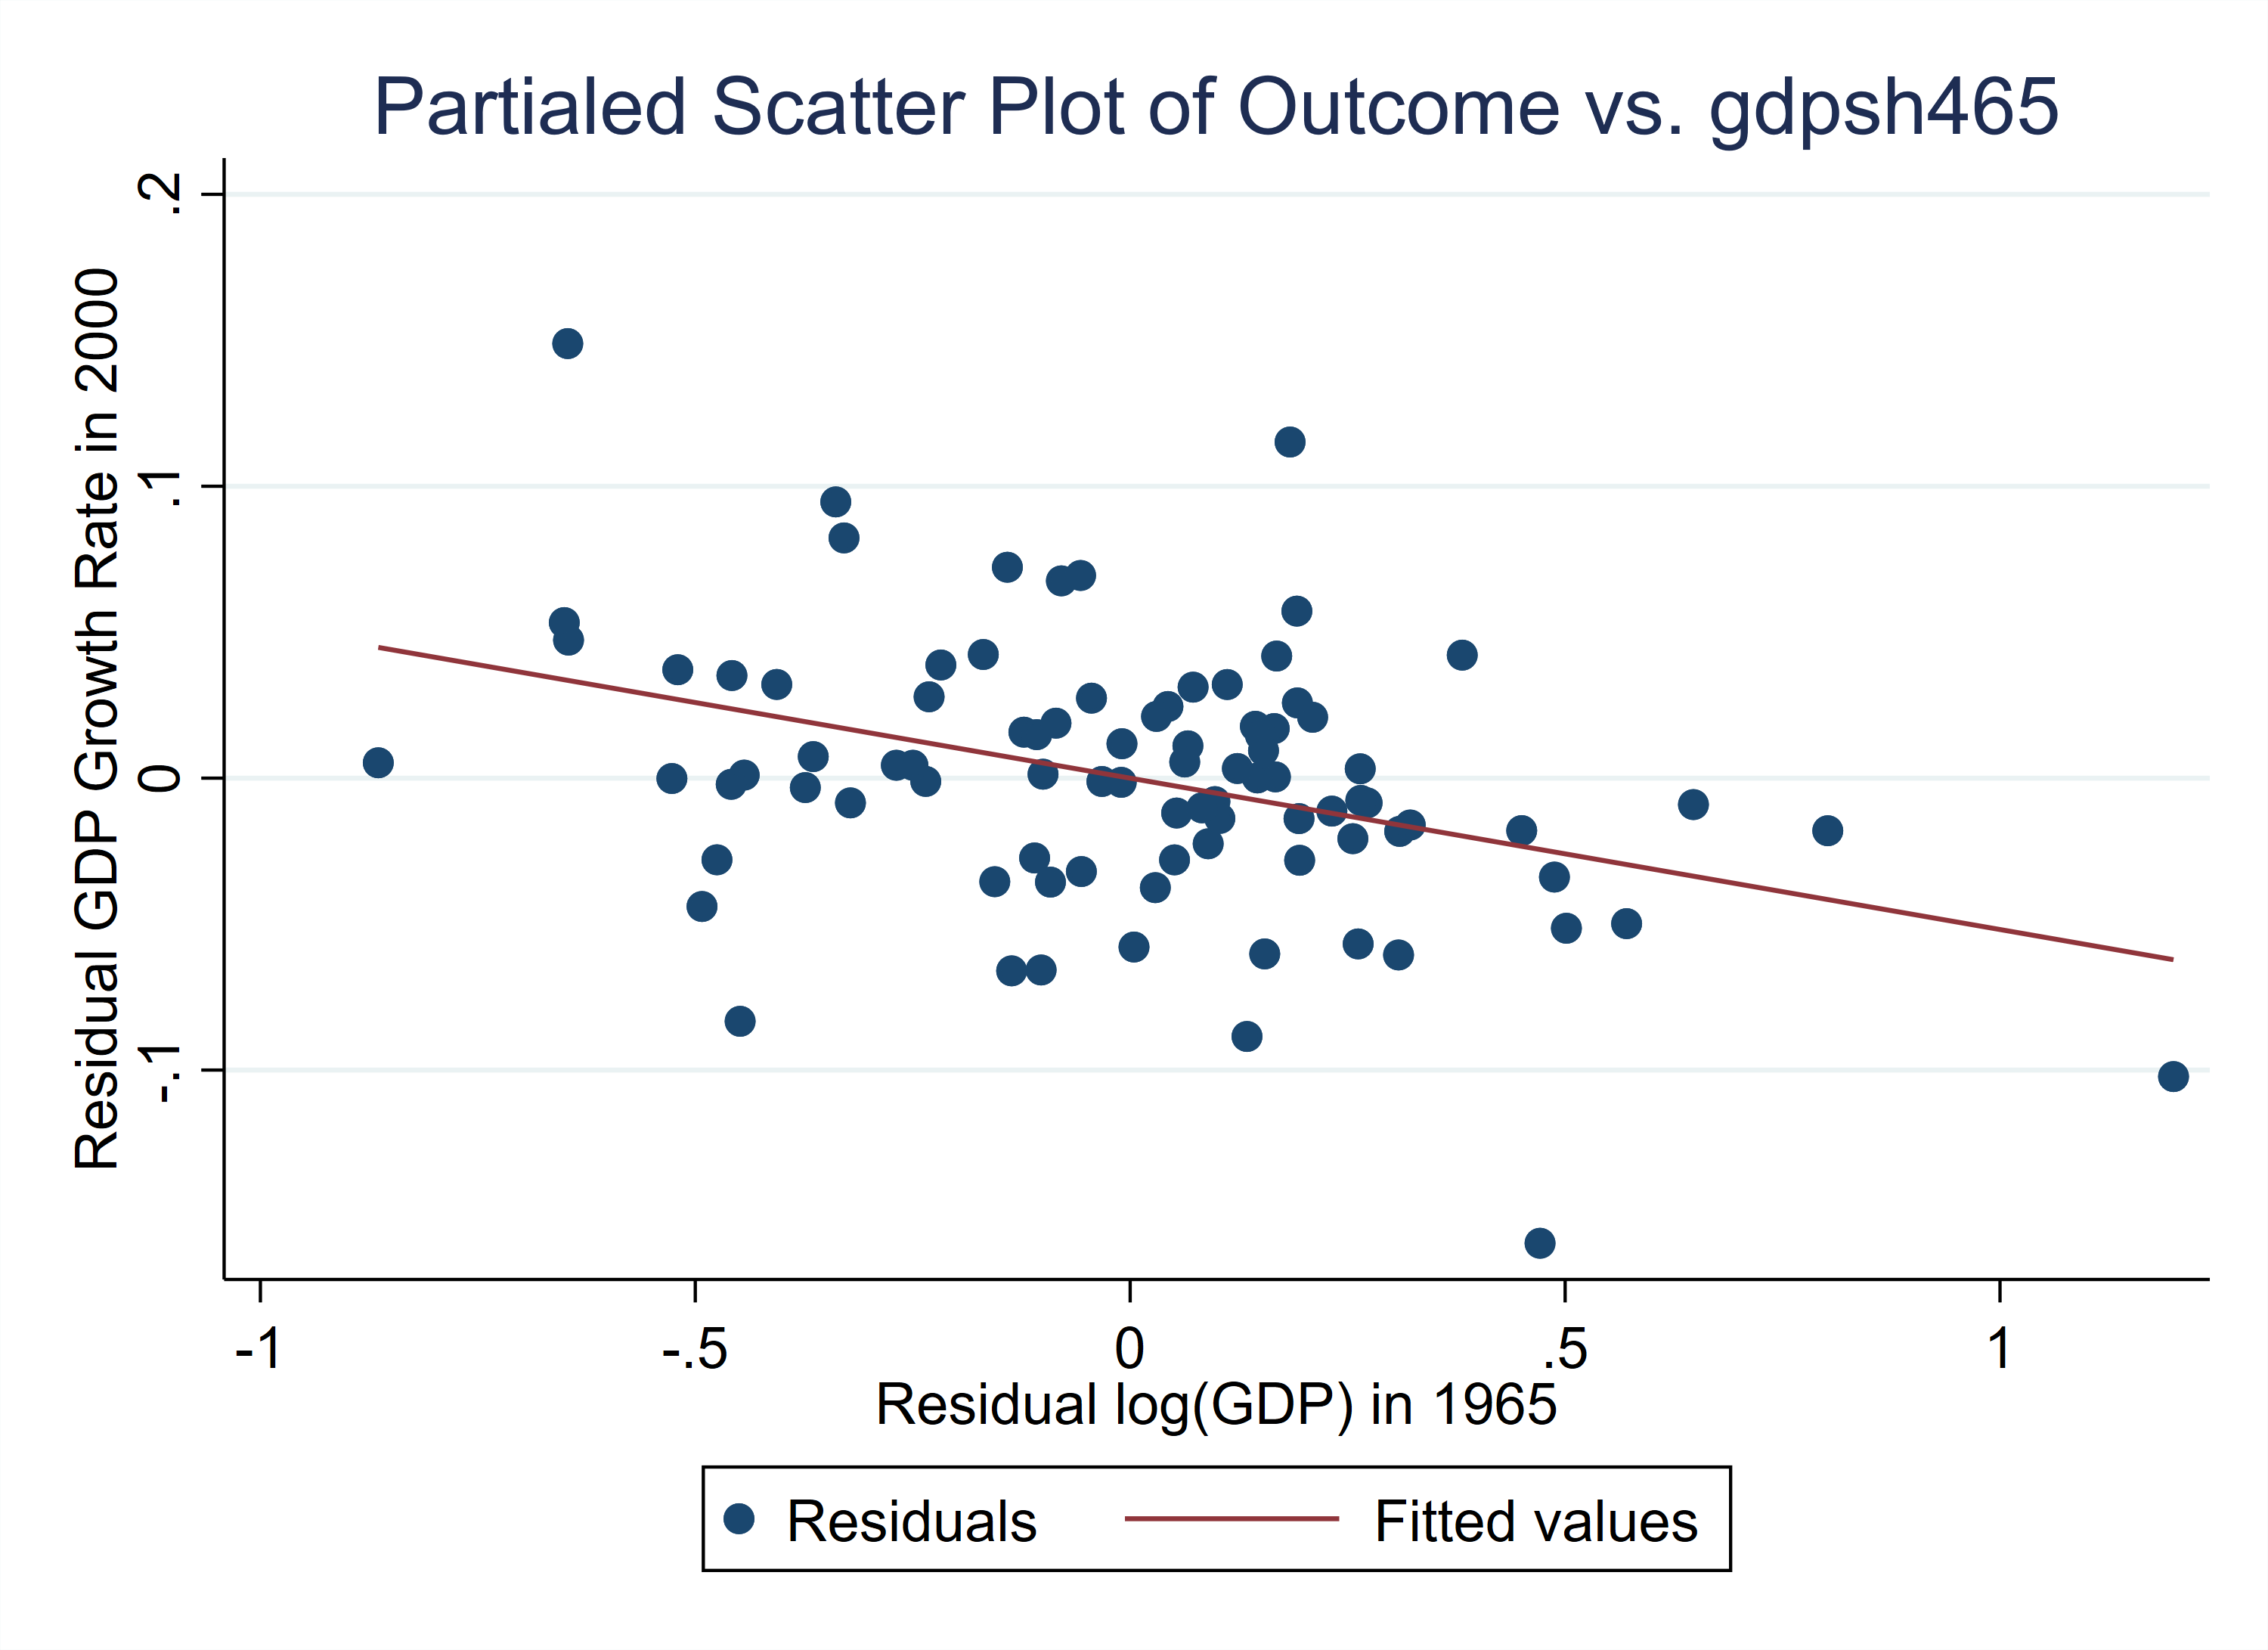
\includegraphics[width=.8\textwidth]{figure/gdp_scatter_r.png}
		\end{figure}
	\end{itemize}
\end{frame}






\title[]  
{R Example}


\author 
{}

%\institute{Institute of Economics, Academia Sinica  \\ Econ, NTU}
%\institute{Institute of Economics, Academia Sinica  \\ IMES/IDAS, NCCU}
\institute{}

%\author 
%{楊子霆 \\ 中研院經濟所}

%\institute 
%{中正大學國際經濟專題研討}




\date
{}


\begin{frame}{}
	\titlepage
\end{frame}






\begin{frame}[fragile]{R Example: Test the Convergence Hypothesis}{Data and Code}
	\begin{itemize}
		\item See \textbf{ML.R}
		\vspace{0.2cm}
		\item Use growth.dta
		\vspace{0.2cm}
		\item Install the following packages:
		\begin{itemize}
			\vspace{0.2cm}
			\item haven
			\item hdm
		\end{itemize}
		
	\end{itemize}
\end{frame}



\begin{frame}[fragile]{R Example: Test the Convergence Hypothesis}{Install Packages}
	\begin{itemize}
		
\begin{lstlisting}
install.packages("hdm") 

library(hdm)
\end{lstlisting}
		
		\item Install and load package \textbf{hdm}
		\vspace{0.2cm}
		\begin{itemize}
			\item This package can help you implement post-double selection method
			
		\end{itemize}
	\end{itemize}
\end{frame}



\begin{frame}[fragile]{R Example: Test the Convergence Hypothesis}{Read Data}
\begin{lstlisting}
GrowthData <- read_dta(paste0(rawdata, "/growth.dta"))

# Checking dimensions of the dataset
dim(GrowthData)

varnames = colnames(GrowthData)
\end{lstlisting}
	\begin{itemize}
		\item \textbf{dim(GrowthData)}: Displays the dimensions of the loaded data, ensuring it is loaded correctly.
		
		\vspace{0.2cm}
		
		\item \textbf{varnames}: Stores the names of all variables in the dataset for reference.
		
	\end{itemize}
\end{frame}






\begin{frame}[fragile]{R Example: Test the Convergence Hypothesis}{Create Sample for Analysis}
\begin{lstlisting}
y = GrowthData[, 1, drop = F]
d = GrowthData[, 2, drop = F]
X = as.matrix(GrowthData)[, -c(1, 2)]
varnames = colnames(GrowthData)
\end{lstlisting}
	\begin{itemize}
		\item Load dataset and define outcome $y$, treatment variable $d$, and covariates $x$
		\begin{itemize}
			\vspace{0.2cm}
			\item \textbf{y}: Dependent variable, representing the first column of the dataset.
			\vspace{0.2cm}
			\item \textbf{d}: Treatment or key independent variable, taken from the second column.
			\vspace{0.2cm}
			\item \textbf{X}: Matrix of covariates, includes all columns except the first two.
		\end{itemize}
		
		
	\end{itemize}
\end{frame}








\begin{frame}[fragile]{R Example: Test the Convergence Hypothesis}{PDS Estimation}
	\begin{itemize}
		
\begin{lstlisting}
doublesel.effect = rlassoEffect(x = X, y = y, d = d, method = "double selection")

summary(doublesel.effect)
\end{lstlisting}
		
		\item Implement double selection estimation and report the treatment effect
		
		
	\end{itemize}
\end{frame}





\begin{frame}[fragile]{R Example: Visualize Data}{Scatter Plot}
\begin{lstlisting}[language=R]
ggplot(GrowthData, aes(x = gdpsh465, y = Outcome)) +
geom_point() +
geom_smooth(method = "lm", se = FALSE, color = "blue") +
labs(title = "GDP Growth Rate (2000) vs. log(GDP) (1965)",
x = "log(GDP) in 1965",
y = "GDP Growth Rate in 2000") +
theme(plot.background = element_rect(fill = "white")) +
scale_x_continuous(breaks = seq(5, 10, by = 1)) +
scale_y_continuous(breaks = seq(-0.1, 0.2, by = 0.1))
\end{lstlisting}
	
	\begin{itemize}
		\item \textbf{ggplot()} 
				\vspace{0.2cm}
		\begin{itemize}
			\item Initializes the plot with `gdpsh465` on the x-axis and `Outcome` on the y-axis.
		\end{itemize}
		\vspace{0.2cm}
		\item \textbf{geom\_point()} 
						\vspace{0.2cm}
		\begin{itemize}
			\item Adds scatter points to the plot.
		\end{itemize}
		
	\end{itemize}
\end{frame}



\begin{frame}[fragile]{R Example: Visualize Data}{Scatter Plot}
\begin{lstlisting}[language=R]
ggplot(GrowthData, aes(x = gdpsh465, y = Outcome)) +
geom_point() +
geom_smooth(method = "lm", se = FALSE, color = "blue") +
labs(title = "GDP Growth Rate (2000) vs. log(GDP) (1965)",
x = "log(GDP) in 1965",
y = "GDP Growth Rate in 2000") +
theme(plot.background = element_rect(fill = "white")) +
scale_x_continuous(breaks = seq(5, 10, by = 1)) +
scale_y_continuous(breaks = seq(-0.1, 0.2, by = 0.1))
\end{lstlisting}
	
	\begin{itemize}
		
		\item \textbf{geom\_smooth(method = "lm")} 
								\vspace{0.2cm}
		\begin{itemize}
			\item Adds a linear regression line without confidence interval shading.
		\end{itemize}
								\vspace{0.2cm}
		\item \textbf{theme(plot.background = ...)} 
						\vspace{0.2cm}
		\begin{itemize}
			\item Sets the background color of the plot to white.
		\end{itemize}
		\vspace{0.2cm}
		\item \textbf{scale\_x\_continuous()} \& \textbf{scale\_y\_continuous()} 
						\vspace{0.2cm}
		
	\begin{itemize}
			\item Controls the axis ticks to match specific intervals.
		\end{itemize}
		\vspace{0.2cm}
		
	\end{itemize}
\end{frame}



\begin{frame}[fragile]{R Example: Visualize Data}{Scatter Plot}
\begin{lstlisting}[language=R]		
ggsave(filename = file.path(pic, "gdp_scatter.png"), width = 10, dpi = 300)
\end{lstlisting}
	
	\begin{itemize}
		
		\item \textbf{ggsave()}
		\vspace{0.2cm} 
		\begin{itemize}
			\item Saves the plot as a PNG image named \texttt{gdp\_scatter.png}.
		\end{itemize}
	\end{itemize}
\end{frame}


\begin{frame}[fragile]{R Example: Visualize Data}{Residuals from Regressions}
\begin{lstlisting}[language=R]
# Step 1: Regress Outcome on controls, extract residuals
model_y <- lm(Outcome ~ bmp1l + freetar + hm65 + sf65 + lifee065 + humanf65 + pop6565, data = GrowthData)
data$res_Outcome <- resid(model_y)

# Step 2: Regress gdpsh465 on controls, extract residuals
model_x <- lm(gdpsh465 ~ bmp1l + freetar + hm65 + sf65 + lifee065 + humanf65 + pop6565, data = GrowthData)
data$res_gdpsh465 <- resid(model_x)
\end{lstlisting}
\end{frame}



\begin{frame}[fragile]{R Example: Visualize Data}{Scatter Plot: residuals}
\begin{lstlisting}[language=R]
ggplot(GrowthData, aes(x = res_gdpsh465, y = res_Outcome)) +
geom_point() +
geom_smooth(method = "lm", se = FALSE, color = "blue") +
labs(title = "Partialed Scatter Plot of Outcome vs. gdpsh465",
x = "Residual log(GDP) in 1965",
y = "Residual GDP Growth Rate in 2000") +
theme(plot.background = element_rect(fill = "white")) +
scale_x_continuous(breaks = seq(-1, 1, by = 0.5)) +
scale_y_continuous(breaks = seq(-0.1, 0.2, by = 0.1))

ggsave(filename = file.path(pic, "gdp_scatter_r.png"), width = 10, dpi = 300)
\end{lstlisting}
\end{frame}





\begin{frame}{Recommended Resources for Self-Learning}
	\begin{itemize}
		\item Machine Learning \& Causal Inference: A Short Course
		\vspace{0.2cm}
		\begin{itemize}
			\item \url{https://www.gsb.stanford.edu/faculty-research/centers-initiatives/sil/research/methods/ai-machine-learning/short-course}
			\vspace{0.2cm}
		\end{itemize}
	
		
		
		
		
	\end{itemize}
\end{frame}



	
\begin{frame}{Recommended Resources for Self-Learning}
	\begin{itemize}
		\item NBER Summer Institute 2013: Econometric Methods for High-Dimensional
		Data
		\vspace{0.2cm}
		\begin{itemize}
			\item \url{https://www.nber.org/econometrics_minicourse_2013/}
	\vspace{0.2cm}
		\end{itemize}
		\item One free textbook: An Introduction to Statistical Learning
		\vspace{0.2cm}
		\begin{itemize}
			\item Website: 
							\vspace{0.2cm} 
					\begin{itemize}
			\item \url{http://faculty.marshall.usc.edu/gareth-james/}
				\vspace{0.2cm}
						\end{itemize}
			\item Video lectures:  
							\vspace{0.2cm} 
								\begin{itemize}
			\url{https://www.youtube.com/playlist?list=PLOg0ngHtcqbPTlZzRHA2ocQZqB1D_qZ5V}
									\end{itemize}
		\end{itemize}

	

	
	\end{itemize}
\end{frame}


\begin{frame}{Recommended Resources for Self-Learning}
\begin{itemize}
	\item the Stata Lasso Page
	\vspace{0.2cm}
	\begin{itemize}
		\item \url{https://statalasso.github.io/}
		\vspace{0.2cm}
	\end{itemize}
	
	
	
\end{itemize}
\end{frame}


\end{document} 